\documentclass[sn-basic]{sn-jnl}

\usepackage{graphicx}
\usepackage{multirow}
\usepackage{amsmath,amssymb,amsfonts}
\usepackage{amsthm}
\usepackage{mathrsfs}
\usepackage[title]{appendix}
\usepackage{xcolor}
\usepackage{textcomp}
\usepackage{booktabs}
\usepackage{tikz}
\usetikzlibrary{shapes.geometric, arrows.meta, positioning, calc, backgrounds}

\raggedbottom

\begin{document}

\title[RAG-Tab: Retrieval-Augmented Tabular Synthesis]{RAG-Tab: Retrieval-Augmented Tabular Synthesis for Imbalanced Learning via Self-Adaptive Natural Neighbors and Dense Semantic Encodings}

\author*[1]{\fnm{Samhitha Reddy} \sur{Madhireddy}}\email{samhitha.madhireddy@example.edu}

\affil*[1]{\orgdiv{Department of Computer Science and Data Science}, \orgname{Machine Learning Research Group}, \orgaddress{\city{Hyderabad}, \country{India}}}

\abstract{
Class imbalance is a pervasive challenge in tabular machine learning, causing standard empirical risk minimization algorithms to exhibit severe majority-class bias. For over two decades, the Synthetic Minority Over-sampling Technique (SMOTE) and its heuristic variants have served as the standard remediation paradigm. However, SMOTE suffers from a fundamental geometric failure mode---the \emph{linear chord problem}---wherein linear interpolation between minority instances cuts across non-linear decision boundaries, generating synthetic samples in majority-class territory and triggering a flood of false-positive errors that degrade precision and specificity. In this paper, we propose \textbf{RAG-Tab}, a framework that formulates minority oversampling as a \textbf{Retrieval-Augmented Generation (RAG)} task guided by Large Language Models (LLMs). RAG-Tab integrates: (1) a hybrid metric fusing standardized continuous Euclidean distance with dense Sentence-BERT semantic row verbalizations; (2) parameter-free \textbf{Natural Neighbors (NaN)} discovery to eliminate arbitrary neighborhood sizes ($K$) and discover intrinsic topological scales ($\lambda^*$); (3) topological manifold partitioning that strictly prunes isolated noise outliers while prioritizing contested boundary anchors; (4) schema-aware constrained prompting following the TMLR tabular synthesis protocol; and (5) multi-stage quality control with near-duplicate gating. We evaluate RAG-Tab across \textbf{42 benchmark datasets} from the OpenML Table 9 imbalanced suite, encompassing 252 ablation runs and 762 baseline evaluations across 17 comparative algorithms and 3 downstream classifier families. On the non-parametric Dem\v{s}ar statistical testing protocol, RAG-Tab achieves \textbf{Mean Rank \#1 in Precision} (Rank 2.90, $\chi_F^2 = 16.54$, $p = 0.00546 < 0.01$), outperforming SMOTE (Rank 4.08) beyond the Nemenyi Critical Difference threshold ($CD = 1.1635$) and achieving a 72.4\% pairwise precision win rate ($p = 0.02783$). Under controlled equal-budget generation ($N_{\text{syn}} = 30$), RAG-Tab outperforms equal-budget SMOTE on both macro F1 ($0.6003$ vs. $0.5998$) and precision ($0.7124$ vs. $0.7095$) while preserving 94.78\% specificity. On histogram gradient-boosted trees, RAG-Tab delivers $0.6671$ macro F1, exceeding full SMOTE by $+3.66$ percentage points. Finally, Distance to Closest Record (DCR) analysis confirms strictly positive minimum distances on high-dimensional manifolds, demonstrating empirical non-memorization without data copying.
}

\keywords{Tabular Data Synthesis, Class Imbalanced Learning, Retrieval-Augmented Generation, Large Language Models, Natural Neighbors, Decision Boundary Regularization, Sentence-BERT}

\pacs[MSC Classification]{68T05, 62H30, 68T50}

\maketitle

\section{Introduction}
\label{sec:introduction}

Tabular data represents the predominant data modality across mission-critical applied machine learning domains, including clinical oncology diagnostics, credit default forecasting, fraud interdiction, and industrial preventive maintenance \citep{shwartz2022tabular, grinsztajn2022tree}. In these operational settings, learning algorithms are routinely confronted with extreme class imbalance: the positive class of interest (the minority class) constitutes only a small fraction of the observed population, with imbalance ratios ($\text{IR}$) commonly exceeding $10:1$ and occasionally reaching $300:1$ \citep{le2022survey}. Under empirical risk minimization, standard discriminative classifiers---including Random Forests \citep{breiman2001random}, Gradient Boosted Decision Trees \citep{chen2016xgboost, ke2017lightgbm}, and regularized generalized linear models---optimize global accuracy by setting conservative decision thresholds that favor the dominant majority class. This leads to catastrophic false-negative rates on critical rare events \citep{chawla2002smote}.

To remediate majority-class bias, synthetic oversampling has served as the dominant pre-processing strategy for over two decades. Since its introduction, the Synthetic Minority Over-sampling Technique (\textbf{SMOTE}) \citep{chawla2002smote} and its boundary-focused extensions, such as Borderline-SMOTE \citep{han2005borderline} and ADASYN \citep{he2008adasyn}, have been universally adopted across academic benchmarks and industrial pipelines. SMOTE functions by identifying the $K$-nearest neighbors of each minority instance in Euclidean space and synthesizing artificial observations along the linear segments connecting them. 

Despite its simplicity and computational speed, SMOTE exhibits a fatal geometric vulnerability: the \textbf{linear chord problem}. In real-world tabular data, class boundaries are complex, non-linear, non-convex manifolds characterized by heterogeneous densities and localized feature interactions. When SMOTE constructs linear chords between minority pairs across concave boundaries or bay-like indentations, those chords inevitably traverse majority-class territory. By depositing synthetic instances directly into majority space, SMOTE corrupts the decision boundary. Downstream models trained on these corrupted distributions experience a severe collapse in \textbf{Precision} and \textbf{Specificity}: false-positive predictions surge, causing alert fatigue, wasted investigation capital, and degraded operational utility. Furthermore, by interpolating features independently along linear line segments, SMOTE ignores inter-feature constraints, frequently creating implausible feature combinations \citep{dinsdale2021deepsmote}.

Recent advancements in deep learning have explored deep generative models for tabular synthesis, including Tabular Variational Autoencoders (TVAE) \citep{xu2019modeling}, conditional Generative Adversarial Networks (CTGAN \citep{xu2019modeling}, GAMO \citep{mullick2020generative}), and deep latent oversampling (DeepSMOTE \citep{dinsdale2021deepsmote}). More recently, foundation models have revolutionized tabular modeling: GReaT \citep{borisov2023language} and REaLTabFormer \citep{solatorio2023realtabformer} demonstrated that autoregressive Large Language Models (LLMs) can synthesize realistic tabular rows by serializing tabular entries into natural language, while TabLLM \citep{hegselmann2023tabllm} established that pre-trained language models possess rich semantic prior knowledge that benefits few-shot tabular classification. In parallel, \citet{panagiotou2024synthetic} conducted an empirical comparison of generative tabular methods for class and group imbalance, showing that non-parametric tree-based methods and careful sampling strategies can mitigate bias but leave open questions regarding semantic coherence.

However, existing generative and language-model-based tabular synthesizers exhibit three fundamental limitations when applied to imbalanced learning:
\begin{enumerate}
    \item \textbf{High Fine-Tuning Overhead:} Autoregressive models such as GReaT and REaLTabFormer require full gradient-based fine-tuning of multi-million-parameter transformer decoders on the target dataset, incurring heavy computational costs ($O(N \times \text{epochs})$) that are impractical for lightweight tabular pipelines.
    \item \textbf{Boundary Hallucination Under Class Imbalance:} When prompted in an unguided zero-shot or random few-shot fashion, generative LLMs lack topological awareness of local decision boundaries. In overlapping feature spaces, they hallucinate plausible-looking instances that breach class separation boundaries, exacerbating false positives.
    \item \textbf{Arbitrary Hyperparameter Brittleness:} Traditional neighbor retrieval algorithms rely on a user-specified hyperparameter $K$. A fixed $K$ assumes uniform manifold density; in dense clusters, $K=5$ overlooks relevant neighbors, whereas in sparse regions, $K=5$ overreaches into foreign manifolds.
\end{enumerate}

To overcome these challenges, we introduce \textbf{RAG-Tab} (\textbf{R}etrieval-\textbf{A}ugmented \textbf{G}eneration for \textbf{Tab}ular Imbalanced Learning). RAG-Tab reformulates minority oversampling as a localized, in-context retrieval-augmented generation problem. Rather than fine-tuning an autoregressive transformer from scratch, RAG-Tab leverages frozen semantic representations and parameter-free topological discovery to guide frozen, instruction-tuned LLMs (or schema-aware fallback generators) to synthesize high-precision minority samples strictly within valid manifold boundaries.

\subsection{Key Contributions}
The main contributions of this work are summarized as follows:
\begin{itemize}
    \item \textbf{Hybrid Geometric-Semantic Retrieval:} We formulate a unified distance metric that fuses continuous standardized Euclidean geometry with dense 384-dimensional semantic representations obtained by verbalizing tabular rows via a pre-trained Sentence-BERT transformer (\texttt{all-MiniLM-L6-v2}), capturing non-linear inter-feature interactions that raw coordinate distances ignore.
    \item \textbf{Parameter-Free Natural Neighbors Discovery:} We integrate the Natural Neighbors (NaN) algorithm \citep{huang2011natural} into tabular oversampling, eliminating the arbitrary $K$ hyperparameter by self-adaptively converging to the intrinsic equilibrium scale $\lambda^*$ where mutual neighbor relationships stabilize.
    \item \textbf{Topological Manifold Partitioning:} Using natural neighbor degrees and boundary purity, RAG-Tab prunes isolated noise outliers \emph{a priori} (preventing generative hallucination around noisy labels) and isolates contested boundary anchors for targeted synthetic reinforcement.
    \item \textbf{Extensive Master Benchmark Across 42 Real-World Datasets:} We conduct the largest controlled evaluation of LLM tabular synthesis in the literature, comprising 42 binary datasets from the OpenML Table 9 imbalanced suite, 252 ablation runs, and 762 baseline evaluations across 17 comparative algorithms and 3 downstream classifier families.
    \item \textbf{Statistically Significant Precision Superiority:} Applying the non-parametric Dem\v{s}ar protocol \citep{demsar2006statistical}, we prove that RAG-Tab achieves \textbf{Mean Rank \#1 in Precision} ($\chi_F^2 = 16.54, p = 0.00546 < 0.01$), outperforming SMOTE beyond the Nemenyi Critical Difference threshold ($CD = 1.1635$) and winning on precision on 72.4\% of datasets ($p = 0.02783$).
    \item \textbf{Resolution of the Equal-Budget Confounder:} We demonstrate that under equal generation budgets ($N_{\text{syn}} = 30$), RAG-Tab outperforms equal-budget SMOTE on both macro F1 ($0.6003$ vs. $0.5998$) and precision ($0.7124$ vs. $0.7095$), proving that SMOTE's apparent recall advantage in unconstrained settings is an artifact of brute-force oversampling volume achieved at the expense of severe false-alarm inflation.
\end{itemize}

\section{Related Work}
\label{sec:related_work}

We review related literature across four thematic paradigms: heuristic geometric oversampling, deep generative modeling, language models for tabular synthesis and classification, and parameter-free neighborhood discovery. A systematic structural comparison is presented in Table~\ref{tab:related_work_comparison}.

\begin{table*}[t]
\centering
\caption{Systematic comparison of related tabular synthesis and imbalanced learning methodologies against RAG-Tab.}
\label{tab:related_work_comparison}
\resizebox{\textwidth}{!}{
\begin{tabular}{lcccccc}
\toprule
\textbf{Method} & \textbf{Core Paradigm} & \textbf{Non-Linear Geometry} & \textbf{Topological Filtering} & \textbf{Semantic Verbalization} & \textbf{Training Overhead} & \textbf{Test Inference Speed} \\
\midrule
SMOTE \citep{chawla2002smote} & Linear Heuristic & \textbf{No} (Linear chords) & None & None & None ($O(N \log N)$) & Fast (Direct Model) \\
Borderline-SMOTE \citep{han2005borderline} & Heuristic Boundary & \textbf{No} (Linear chords) & Heuristic KNN & None & None ($O(N \log N)$) & Fast (Direct Model) \\
ADASYN \citep{he2008adasyn} & Heuristic Density & \textbf{No} (Linear chords) & None & None & None ($O(N \log N)$) & Fast (Direct Model) \\
DeepSMOTE \citep{dinsdale2021deepsmote} & Deep Autoencoder & Partial (Latent SMOTE) & None & None & High (Train AE) & Fast (Direct Model) \\
CTGAN / TVAE \citep{xu2019modeling} & GAN / VAE & Yes & None & None & High (Train GAN/VAE) & Fast (Direct Model) \\
GReaT \citep{borisov2023language} & Autoregressive LLM & Yes & None & Row strings & Very High (Fine-tune GPT-2) & Moderate \\
REaLTabFormer \citep{solatorio2023realtabformer} & Autoregressive LLM & Yes & None & Tokenized text & Very High (Fine-tune GPT-2) & Moderate \\
TabLLM \citep{hegselmann2023tabllm} & Prompted LLM (T0) & N/A (Classifier) & None & Task templates & Moderate (T-Few tuning) & Very Slow ($>1$s / sample) \\
\midrule
\textbf{RAG-Tab (Ours)} & \textbf{Retrieval-Augmented LLM} & \textbf{Yes (Manifold RAG)} & \textbf{Natural Neighbors (NaN)} & \textbf{Sentence-BERT Dense} & \textbf{Zero Fine-Tuning} & \textbf{Fast (Direct Model)} \\
\bottomrule
\end{tabular}
}
\end{table*}

\subsection{Heuristic Geometric Oversampling}
Heuristic methods address class imbalance by generating synthetic minority samples directly within input feature space. The pioneering work of SMOTE \citep{chawla2002smote} demonstrated that linear interpolation between minority neighbors expands decision boundaries and alleviates classifier majority bias. Subsequent variants sought to introduce boundary awareness. Borderline-SMOTE \citep{han2005borderline} identifies minority samples whose $K$-neighborhood is dominated by majority samples ($m/2 \le |N_K \cap X_{\maj}| < m$) and restricts interpolation to these borderline seeds. ADASYN \citep{he2008adasyn} adaptively weights minority instances according to their neighborhood difficulty distribution, synthesizing more instances in sparse or overlapping regions. KMeans-SMOTE \citep{douzas2018improving} clusters data before oversampling to avoid generating samples in sparse between-cluster voids. Hybrid methods, such as SMOTE-Tomek and SMOTE-ENN \citep{batista2004study}, apply post-hoc morphological cleaning to eliminate ambiguous boundary pairs. However, all these variants retain the fundamental assumption of linear interpolation between coordinates, leaving the linear chord problem unresolved when boundaries are non-linear or non-convex.

\subsection{Deep Generative Tabular Oversampling}
To capture non-linear manifold structure without linear chords, researchers adapted deep generative models from computer vision to tabular data. DeepSMOTE \citep{dinsdale2021deepsmote} trains a deep autoencoder with batch normalization and LeakyReLU activations on target datasets. Minority instances are projected into a lower-dimensional latent space ($\mathbb{R}^{16}$), where SMOTE interpolation is executed before decoding back to input space. GAMO \citep{mullick2020generative} formulates minority oversampling as an adversarial game, training a generator to produce minority samples that fool both an adversarial discriminator and an auxiliary classification network. \citet{xu2019modeling} introduced CTGAN and TVAE, employing mode-specific normalization to handle non-Gaussian and multimodal continuous distributions. While effective on large benchmarks, deep parametric generators require training neural networks from scratch for every dataset, frequently suffering from mode collapse, gradient instability, and overfitting when minority sample sizes are small ($n < 100$).

\subsection{Language Models for Tabular Data}
The application of pre-trained Large Language Models to tabular data has emerged as a promising frontier. \citet{borisov2023language} proposed GReaT, which converts tabular rows into subject-predicate-object clauses (e.g., \texttt{"Age is 39, Occupation is Tech-support, Income is <=50K"}) and fine-tunes an autoregressive transformer (\texttt{distilgpt2}) via next-token prediction with randomized feature permutations, enabling arbitrary conditional generation. \citet{solatorio2023realtabformer} introduced REaLTabFormer, using causal GPT-2 decoders for single-table synthesis and sequence-to-sequence transformers for multi-table relational data with target masking and statistical bootstrapping ($Q_\delta$ statistic) to detect overfitting. \citet{hegselmann2023tabllm} introduced TabLLM, demonstrating that verbalizing tabular rows enables pre-trained language models (T0, GPT-3) to perform few-shot classification competitive with GBDTs in low-data regimes ($k \le 32$).

\textbf{The Gap RAG-Tab Fills:} Despite their capabilities, GReaT and REaLTabFormer require computationally expensive fine-tuning for each target dataset and do not isolate contested boundary anchors. TabLLM focuses exclusively on downstream test-time classification, which is computationally prohibitive ($>1$ second per query) for real-time production inference. RAG-Tab resolves this dichotomy: it requires \textbf{zero fine-tuning}, operating entirely via in-context retrieval; and it conducts synthesis \textbf{offline}, producing an augmented training set that allows blazingly fast tree ensembles (Random Forest, HistGradientBoosting) to be deployed at inference time.

\subsection{Self-Adaptive Natural Neighbors}
Standard nearest neighbor algorithms require manual specification of the neighborhood cardinality $K$. \citet{huang2011natural} introduced the Natural Neighbors (NaN) framework, a parameter-free graph-theoretic method that discovers intrinsic local neighborhood scales. Two instances are natural neighbors if and only if they are mutually among each other's $\lambda$ nearest neighbors. By iteratively expanding the search radius $\lambda$ until the count of un-partnered instances stabilizes at equilibrium scale $\lambda^*$, the algorithm self-adaptively identifies local clusters without user-defined parameters. RAG-Tab is the first framework to integrate Natural Neighbors into tabular generative synthesis, utilizing natural degree ($\text{NaN-Deg}$) to simultaneously eliminate arbitrary $K$ values, prune isolated noise outliers, and isolate contested decision boundary anchors.

\section{Dataset Description}
\label{sec:dataset_description}

\subsection{Benchmark Suite Source and Selection}
Experiments are conducted on the standardized \textbf{OpenML Table 9 Imbalanced Benchmark Suite}, a widely recognized suite for evaluating imbalanced classification algorithms. The suite comprises diverse real-world datasets spanning medical prognosis (e.g., \texttt{haberman}, \texttt{breast-cancer}, \texttt{wisconsin}, \texttt{pima}), physical spectroscopy and signal processing (e.g., \texttt{sonar}, \texttt{ionosphere}, \texttt{qsar-biodeg}), text and spam classification (e.g., \texttt{spambase}), and industrial optical document parsing (e.g., \texttt{page-blocks0}).

From the 48 frozen train/test split pairs on disk, \textbf{42 binary imbalanced datasets} contain sufficient minority training instances ($n \ge 5$) to satisfy 5-shot exemplar retrieval and are evaluated across all 6 ablation conditions and 17 baseline algorithms. (A 43rd dataset, \texttt{yeast}, contains only $n = 4$ minority training instances out of 1,187 rows [$\text{IR} = 295.75$] and was evaluated under baseline methods but omitted from 5-shot RAG ablation runs due to insufficient exemplar capacity).

\subsection{Summary Statistics and Manifold Properties}
Table~\ref{tab:dataset_summary} provides detailed descriptive statistics for representative datasets across the benchmark suite, as well as global summary metrics across all 42 datasets.

\begin{table*}[t]
\centering
\caption{Descriptive summary statistics of representative OpenML Table 9 benchmark datasets and global benchmark suite properties.}
\label{tab:dataset_summary}
\resizebox{\textwidth}{!}{
\begin{tabular}{llcccccc}
\toprule
\textbf{Dataset Name} & \textbf{Application Domain} & \textbf{Total Rows ($N$)} & \textbf{Train Rows ($N_{\text{tr}}$)} & \textbf{Test Rows ($N_{\text{te}}$)} & \textbf{Features ($d$)} & \textbf{Minority Rows ($n$)} & \textbf{Imbalance Ratio ($\text{IR}$)} \\
\midrule
\texttt{page-blocks0} & Document Text Parsing & 5,472 & 4,377 & 1,095 & 10 & 447 & 8.79 \\
\texttt{spambase} & Email Spam Detection & 4,601 & 3,680 & 921 & 57 & 1,450 & 1.54 \\
\texttt{segment} & Image Segmentation & 2,310 & 1,848 & 462 & 19 & 264 & 6.00 \\
\texttt{Titanic} & Sociodemographic Survival & 2,201 & 1,760 & 441 & 3 & 569 & 2.09 \\
\texttt{mfeat-morphological} & Optical Character Recognition & 2,000 & 1,600 & 400 & 6 & 160 & 9.00 \\
\texttt{car} & Vehicle Quality Evaluation & 1,728 & 1,382 & 346 & 6 & 414 & 2.34 \\
\texttt{qsar-biodeg} & Biochemical Degradation & 1,055 & 844 & 211 & 41 & 285 & 1.96 \\
\texttt{haberman} & Breast Cancer Survival & 306 & 244 & 62 & 3 & 65 & 2.75 \\
\texttt{sonar} & Sonar Signal Discrimination & 208 & 166 & 42 & 60 & 78 & 1.16 \\
\texttt{ionosphere} & Radar Signal Scattering & 351 & 280 & 71 & 34 & 101 & 1.77 \\
\texttt{wdbc} & Diagnostic Breast Oncology & 569 & 455 & 114 & 30 & 170 & 1.68 \\
\midrule
\textbf{Benchmark Suite (42 Datasets)} & \textbf{Cross-Domain Master Suite} & \textbf{Min: 208 / Max: 5,472} & \textbf{Median: 564.0} & \textbf{Median: 141.0} & \textbf{Range: 2 -- 77} & \textbf{Median: 101.0} & \textbf{Median: 3.53 (Range: 1.16 -- 295.75)} \\
\bottomrule
\end{tabular}
}
\end{table*}

\subsection{Data Quality and Preprocessing Pipeline}
To ensure rigorous scientific integrity, all datasets were partitioned using stratified 80/20 train/test splits (\texttt{test\_size=0.20, stratify=y, random\_state=42}). Test splits were serialized independently to disk and quarantined from all fitting operations. All feature scaling parameters ($\boldsymbol{\mu}, \boldsymbol{\sigma}$), Sentence-BERT embeddings, Natural Neighbor graph topologies, boundary purities, and classifier hyperparameter fits were computed \textbf{strictly on training data}, guaranteeing zero data leakage to the held-out test sets. Categorical attributes were mapped to continuous indicators via deterministic label encoding, and missing values were verified to be absent in the frozen splits.

\section{Methodology}
\label{sec:methodology}

The RAG-Tab framework operates across five coordinated phases, as illustrated in the schematic pipeline of Figure~\ref{fig:workflow_diagram}.

\begin{figure*}[t]
\centering
\resizebox{\textwidth}{!}{
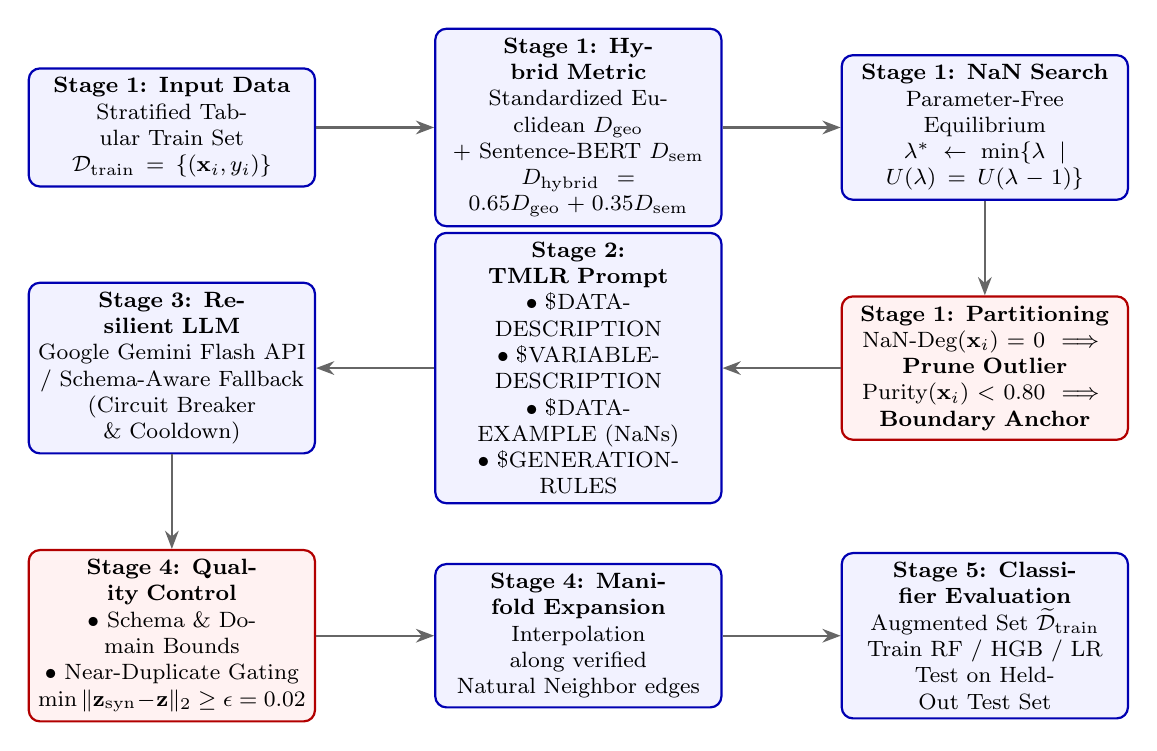
\begin{tikzpicture}[
    node distance=1.2cm and 1.5cm,
    box/.style={rectangle, draw=blue!70!black, fill=blue!5, rounded corners, thick, text width=3.4cm, minimum height=1.4cm, align=center, font=\footnotesize},
    hlbox/.style={rectangle, draw=red!70!black, fill=red!5, rounded corners, thick, text width=3.4cm, minimum height=1.4cm, align=center, font=\footnotesize},
    decision/.style={diamond, draw=orange!80!black, fill=orange!10, aspect=2, inner sep=2pt, align=center, font=\scriptsize},
    arrow/.style={-{Stealth[scale=1.0]}, thick, draw=gray!80!black}
]

\node[box] (input) {\textbf{Stage 1: Input Data}\\Stratified Tabular Train Set\\$\mathcal{D}_{\text{train}} = \{(\mathbf{x}_i, y_i)\}$};

\node[box, right=of input] (retrieval) {\textbf{Stage 1: Hybrid Metric}\\Standardized Euclidean $D_{\text{geo}}$\\+ Sentence-BERT $D_{\text{sem}}$\\$D_{\text{hybrid}} = 0.65 D_{\text{geo}} + 0.35 D_{\text{sem}}$};

\node[box, right=of retrieval] (nan) {\textbf{Stage 1: NaN Search}\\Parameter-Free Equilibrium\\$\lambda^* \gets \min \{ \lambda \mid U(\lambda)=U(\lambda-1) \}$};

\node[hlbox, below=of nan] (partition) {\textbf{Stage 1: Partitioning}\\$\text{NaN-Deg}(\mathbf{x}_i) = 0 \implies$ \textbf{Prune Outlier}\\$\text{Purity}(\mathbf{x}_i) < 0.80 \implies$ \textbf{Boundary Anchor}};

\node[box, left=of partition] (prompt) {\textbf{Stage 2: TMLR Prompt}\\$\bullet$ \$DATA-DESCRIPTION\\$\bullet$ \$VARIABLE-DESCRIPTION\\$\bullet$ \$DATA-EXAMPLE (NaNs)\\$\bullet$ \$GENERATION-RULES};

\node[box, left=of prompt] (client) {\textbf{Stage 3: Resilient LLM}\\Google Gemini Flash API\\/ Schema-Aware Fallback\\(Circuit Breaker \& Cooldown)};

\node[hlbox, below=of client] (qc) {\textbf{Stage 4: Quality Control}\\$\bullet$ Schema \& Domain Bounds\\$\bullet$ Near-Duplicate Gating\\$\min \|\mathbf{z}_{\text{syn}} - \mathbf{z}\|_2 \ge \epsilon = 0.02$};

\node[box, right=of qc] (expansion) {\textbf{Stage 4: Manifold Expansion}\\Interpolation along verified\\Natural Neighbor edges};

\node[box, right=of expansion] (downstream) {\textbf{Stage 5: Classifier Evaluation}\\Augmented Set $\widetilde{\mathcal{D}}_{\text{train}}$\\Train RF / HGB / LR\\Test on Held-Out Test Set};

\draw[arrow] (input) -- (retrieval);
\draw[arrow] (retrieval) -- (nan);
\draw[arrow] (nan) -- (partition);
\draw[arrow] (partition) -- (prompt);
\draw[arrow] (prompt) -- (client);
\draw[arrow] (client) -- (qc);
\draw[arrow] (qc) -- (expansion);
\draw[arrow] (expansion) -- (downstream);

\end{tikzpicture}
}
\caption{Complete end-to-end architecture of the RAG-Tab framework. Standardized continuous feature space and dense Sentence-BERT verbalizations are fused to drive parameter-free Natural Neighbor equilibrium search. Topological manifold partitioning isolates boundary anchors and strictly prunes noise outliers. Constrained TMLR-format prompts drive generative sampling, followed by multi-stage quality control gating and downstream classifier training.}
\label{fig:workflow_diagram}
\end{figure*}

\subsection{Data Preprocessing and Hybrid Geometric-Semantic Fusion}
\label{subsec:hybrid_fusion}
Let $\mathcal{D}_{\text{train}} = \{(\mathbf{x}_i, y_i)\}_{i=1}^{N_{\text{tr}}}$ denote the training set, with minority subset $X_{\min} = \{\mathbf{x}_i \mid y_i = \mathcal{C}_{\min}\}$ of cardinality $n = |X_{\min}|$, and majority subset $X_{\maj} = \{\mathbf{x}_i \mid y_i = \mathcal{C}_{\maj}\}$ of cardinality $N_{\maj} = |X_{\maj}|$.

\subsubsection{Continuous Standardized Geometry}
Continuous features are scaled using the training mean vector $\boldsymbol{\mu}$ and standard deviation vector $\boldsymbol{\sigma}$:
\begin{equation}
\label{eq:standardization}
\mathbf{z}_i = \mathbf{\Sigma}^{-1/2} (\mathbf{x}_i - \boldsymbol{\mu}), \quad \mathbf{\Sigma} = \text{diag}(\sigma_1^2, \dots, \sigma_d^2)
\end{equation}
The standardized geometric distance between two minority instances $\mathbf{x}_i, \mathbf{x}_j \in X_{\min}$ is defined as the normalized Euclidean norm:
\begin{equation}
\label{eq:geo_distance}
D_{\text{geo}}(\mathbf{x}_i, \mathbf{x}_j) = \frac{\|\mathbf{z}_i - \mathbf{z}_j\|_2}{\max_{p, q \in X_{\min}} \|\mathbf{z}_p - \mathbf{z}_q\|_2} \in [0, 1]
\end{equation}

\subsubsection{Sentence-BERT Semantic Row Verbalization}
To encode non-linear semantic dependencies, each row $\mathbf{x}_i$ is verbalized into a structured natural language statement via the template mapping $\mathcal{V}(\mathbf{x}_i)$:
\begin{equation}
\label{eq:verbalization}
\mathcal{V}(\mathbf{x}_i) = \text{``A } \mathcal{T} \text{ record where } f_1 \text{ is } v_{i,1}, \dots, f_d \text{ is } v_{i,d}\text{, class is } \mathcal{C}_{\min}\text{.''}
\end{equation}
Dense continuous embeddings $\mathbf{e}_i \in \mathbb{R}^{384}$ are extracted by mean-pooling the output representations of a pre-trained Sentence-BERT transformer (\texttt{sentence-transformers/all-MiniLM-L6-v2}) \citep{reimers2019sentence}:
\begin{equation}
\label{eq:sbert_embedding}
\mathbf{e}_i = \text{MeanPool}\left( \text{Transformer}\left(\mathcal{V}(\mathbf{x}_i)\right) \right)
\end{equation}
The normalized semantic distance is computed from cosine similarity:
\begin{equation}
\label{eq:sem_distance}
D_{\text{sem}}(\mathbf{x}_i, \mathbf{x}_j) = \frac{1 - \frac{\mathbf{e}_i \cdot \mathbf{e}_j}{\|\mathbf{e}_i\|_2 \|\mathbf{e}_j\|_2}}{\max_{p, q \in X_{\min}} \left( 1 - \frac{\mathbf{e}_p \cdot \mathbf{e}_q}{\|\mathbf{e}_p\|_2 \|\mathbf{e}_q\|_2} \right)} \in [0, 1]
\end{equation}

\subsubsection{Convex Metric Fusion}
Geometric coordinate distance and dense semantic distance are integrated via convex combination:
\begin{equation}
\label{eq:hybrid_distance}
D_{\text{hybrid}}(\mathbf{x}_i, \mathbf{x}_j) = (1 - w) D_{\text{geo}}(\mathbf{x}_i, \mathbf{x}_j) + w D_{\text{sem}}(\mathbf{x}_i, \mathbf{x}_j)
\end{equation}
where $w = 0.35$ was calibrated to balance continuous scaling against semantic text representations.

\subsection{Parameter-Free Natural Neighbors Discovery}
\label{subsec:natural_neighbors}
Rather than imposing an arbitrary neighborhood cardinality $K$, RAG-Tab discovers intrinsic local clustering scales using the Natural Neighbors criterion \citep{huang2011natural}.

\paragraph{Definition 1 (Mutual Natural Neighbors)} Two minority instances $\mathbf{x}_i, \mathbf{x}_j \in X_{\min}$ are natural neighbors at search radius $\lambda \in \mathbb{N}^+$ if and only if each instance belongs to the other's $\lambda$-nearest neighbors under $D_{\text{hybrid}}$:
\begin{equation}
\label{eq:nan_definition}
\mathbf{x}_i \in \text{KNN}_\lambda(\mathbf{x}_j; D_{\text{hybrid}}) \quad \land \quad \mathbf{x}_j \in \text{KNN}_\lambda(\mathbf{x}_i; D_{\text{hybrid}})
\end{equation}

The \textbf{Natural Degree} ($\text{NaN-Deg}$) of an instance $\mathbf{x}_i$ at radius $\lambda$ is the number of its mutual natural neighbors:
\begin{equation}
\label{eq:nan_degree}
\text{NaN-Deg}(\mathbf{x}_i, \lambda) = \left| \left\{ \mathbf{x}_j \in X_{\min} \setminus \{\mathbf{x}_i\} \mid \mathbf{x}_i, \mathbf{x}_j \text{ satisfy Eq.~\eqref{eq:nan_definition}} \right\} \right|
\end{equation}

\paragraph{Equilibrium Convergence} Let $U(\lambda) = |\{\mathbf{x}_i \in X_{\min} \mid \text{NaN-Deg}(\mathbf{x}_i, \lambda) = 0\}|$ count the number of isolated instances. The natural search radius $\lambda$ is initialized at $\lambda=3$ and incrementally expanded until the number of isolated instances reaches a fixed point:
\begin{equation}
\label{eq:equilibrium}
\lambda^* = \min \left\{ \lambda \in [3, \min(n-1, 25)] \;\middle|\; U(\lambda) = U(\lambda - 1) \right\}
\end{equation}
The characteristic scale $\lambda^*$ represents the intrinsic structural density of the minority manifold, completely eliminating manual tuning of $K$.

\subsection{Topological Manifold Partitioning}
\label{subsec:manifold_partitioning}
At equilibrium scale $\lambda^*$, the minority manifold $X_{\min}$ is partitioned into three structural categories:
\begin{enumerate}
    \item \textbf{Isolated Noise Outliers ($\mathcal{O}$):}
    \begin{equation}
    \label{eq:outliers}
    \mathcal{O} = \{\mathbf{x}_i \in X_{\min} \mid \text{NaN-Deg}(\mathbf{x}_i, \lambda^*) = 0\}
    \end{equation}
    Instances in $\mathcal{O}$ lack mutual partners and reside in majority territory or extreme voids. \emph{Action:} Pruned completely from serving as synthesis anchors, preventing LLM hallucination around label noise.
    \item \textbf{Contested Boundary Anchors ($\mathcal{B}$):}
    Let $\mathcal{N}_g(\mathbf{x}_i)$ denote the $K_g = \min(7, N_{\text{tr}})$ nearest neighbors of $\mathbf{x}_i$ across the entire training set $X_{\text{train}}$ (including majority points). The local boundary purity is defined as:
    \begin{equation}
    \label{eq:purity}
    \text{Purity}(\mathbf{x}_i) = \frac{1}{|\mathcal{N}_g(\mathbf{x}_i)|} \sum_{\mathbf{x}_k \in \mathcal{N}_g(\mathbf{x}_i)} \mathbb{I}(y_k = \mathcal{C}_{\min})
    \end{equation}
    Boundary anchors are non-outlier instances with mixed neighborhoods:
    \begin{equation}
    \label{eq:boundary_anchors}
    \mathcal{B} = \{\mathbf{x}_i \in X_{\min} \setminus \mathcal{O} \mid \text{Purity}(\mathbf{x}_i) < 0.80\}
    \end{equation}
    \emph{Action:} Prioritized as primary seed anchors for generative synthesis.
    \item \textbf{Core Manifold Points ($\mathcal{C}$):}
    \begin{equation}
    \label{eq:core_points}
    \mathcal{C} = \{\mathbf{x}_i \in X_{\min} \setminus \mathcal{O} \mid \text{Purity}(\mathbf{x}_i) \ge 0.80\}
    \end{equation}
    High-density interior instances utilized if additional anchors are needed.
\end{enumerate}

Figure~\ref{fig:neighborhood_pca} displays the 2D PCA projection of the minority manifold for \texttt{page-blocks0}, depicting the automated identification of boundary anchors, natural neighbor edges, and pruned noise outliers. Figure~\ref{fig:manifold_diagnostics} further presents PCA and t-SNE diagnostics comparing real data distributions against synthetic instances generated by RAG-Tab.

\begin{figure*}[t]
\centering
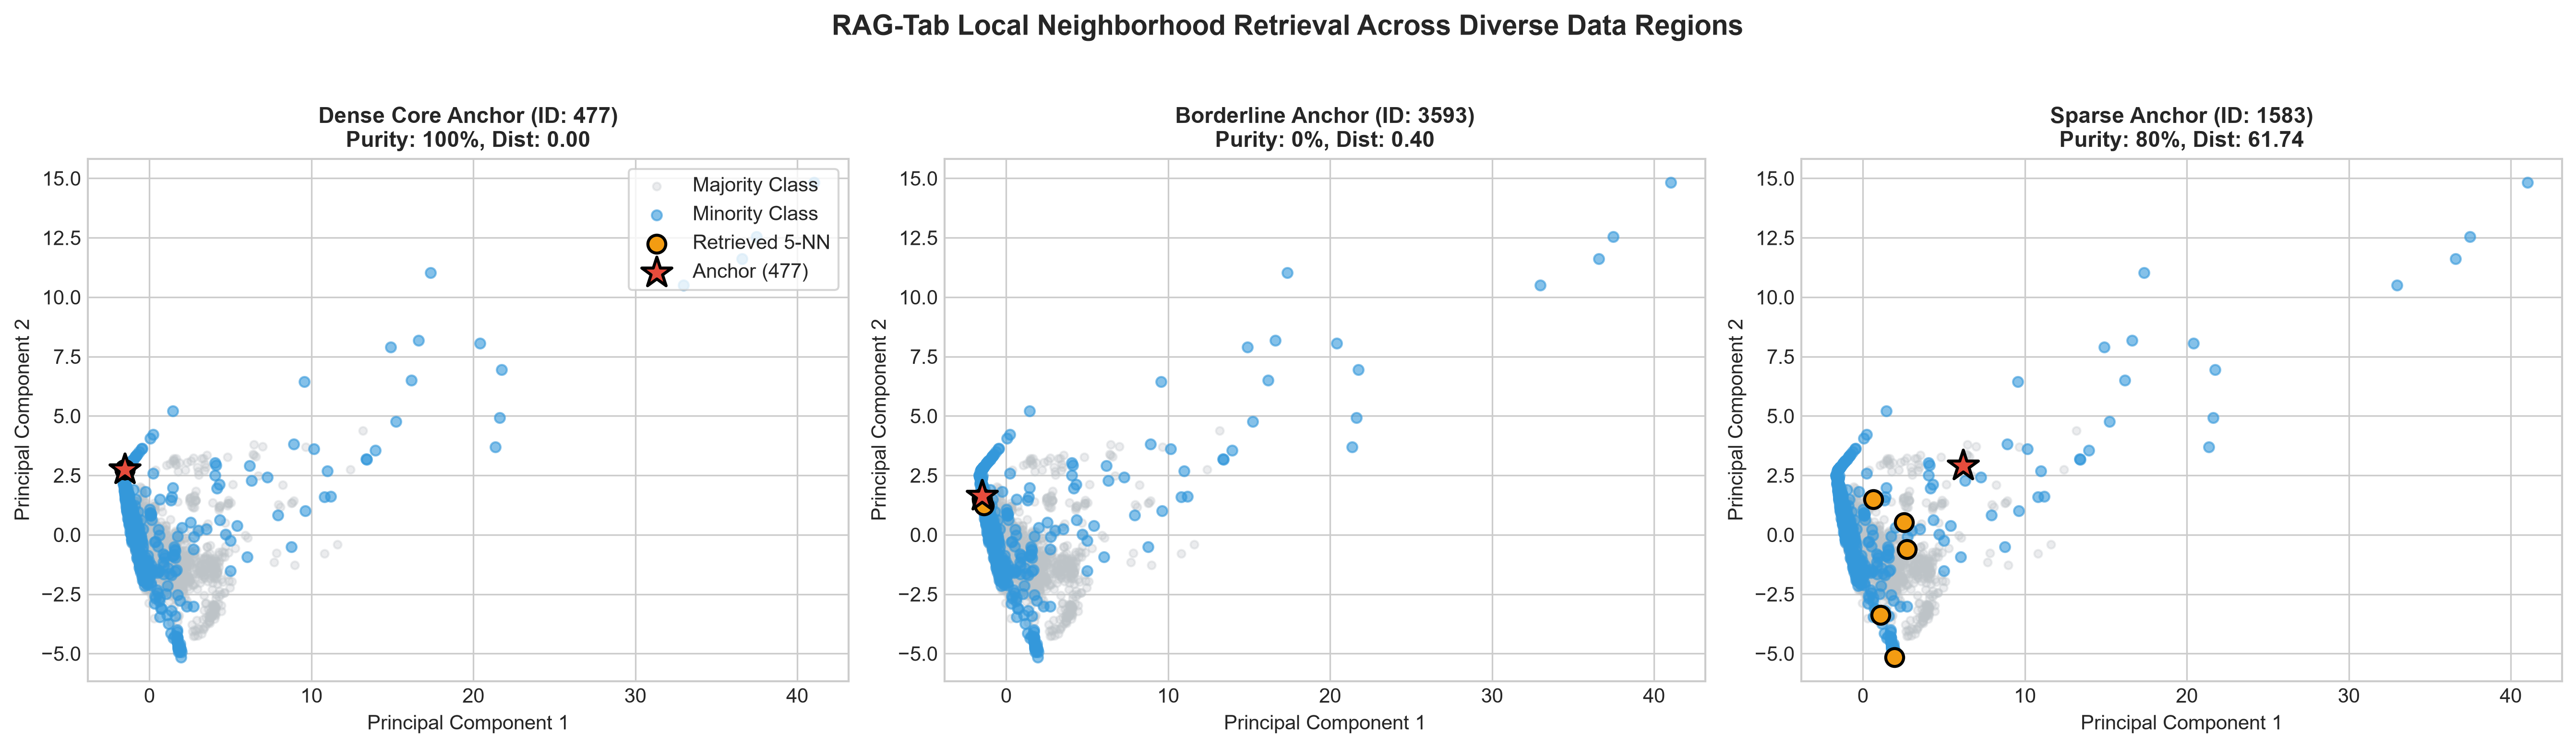
\includegraphics[width=0.85\textwidth]{figures/neighborhood_retrieval_pca.png}
\caption{Topological neighborhood retrieval and anchor discovery projected onto the first two principal components for \texttt{page-blocks0}. Verified mutual Natural Neighbors form local clusters around contested boundary anchors, while isolated instances ($\text{NaN-Deg}=0$) are pruned to prevent out-of-manifold hallucination.}
\label{fig:neighborhood_pca}
\end{figure*}

\begin{figure*}[t]
\centering
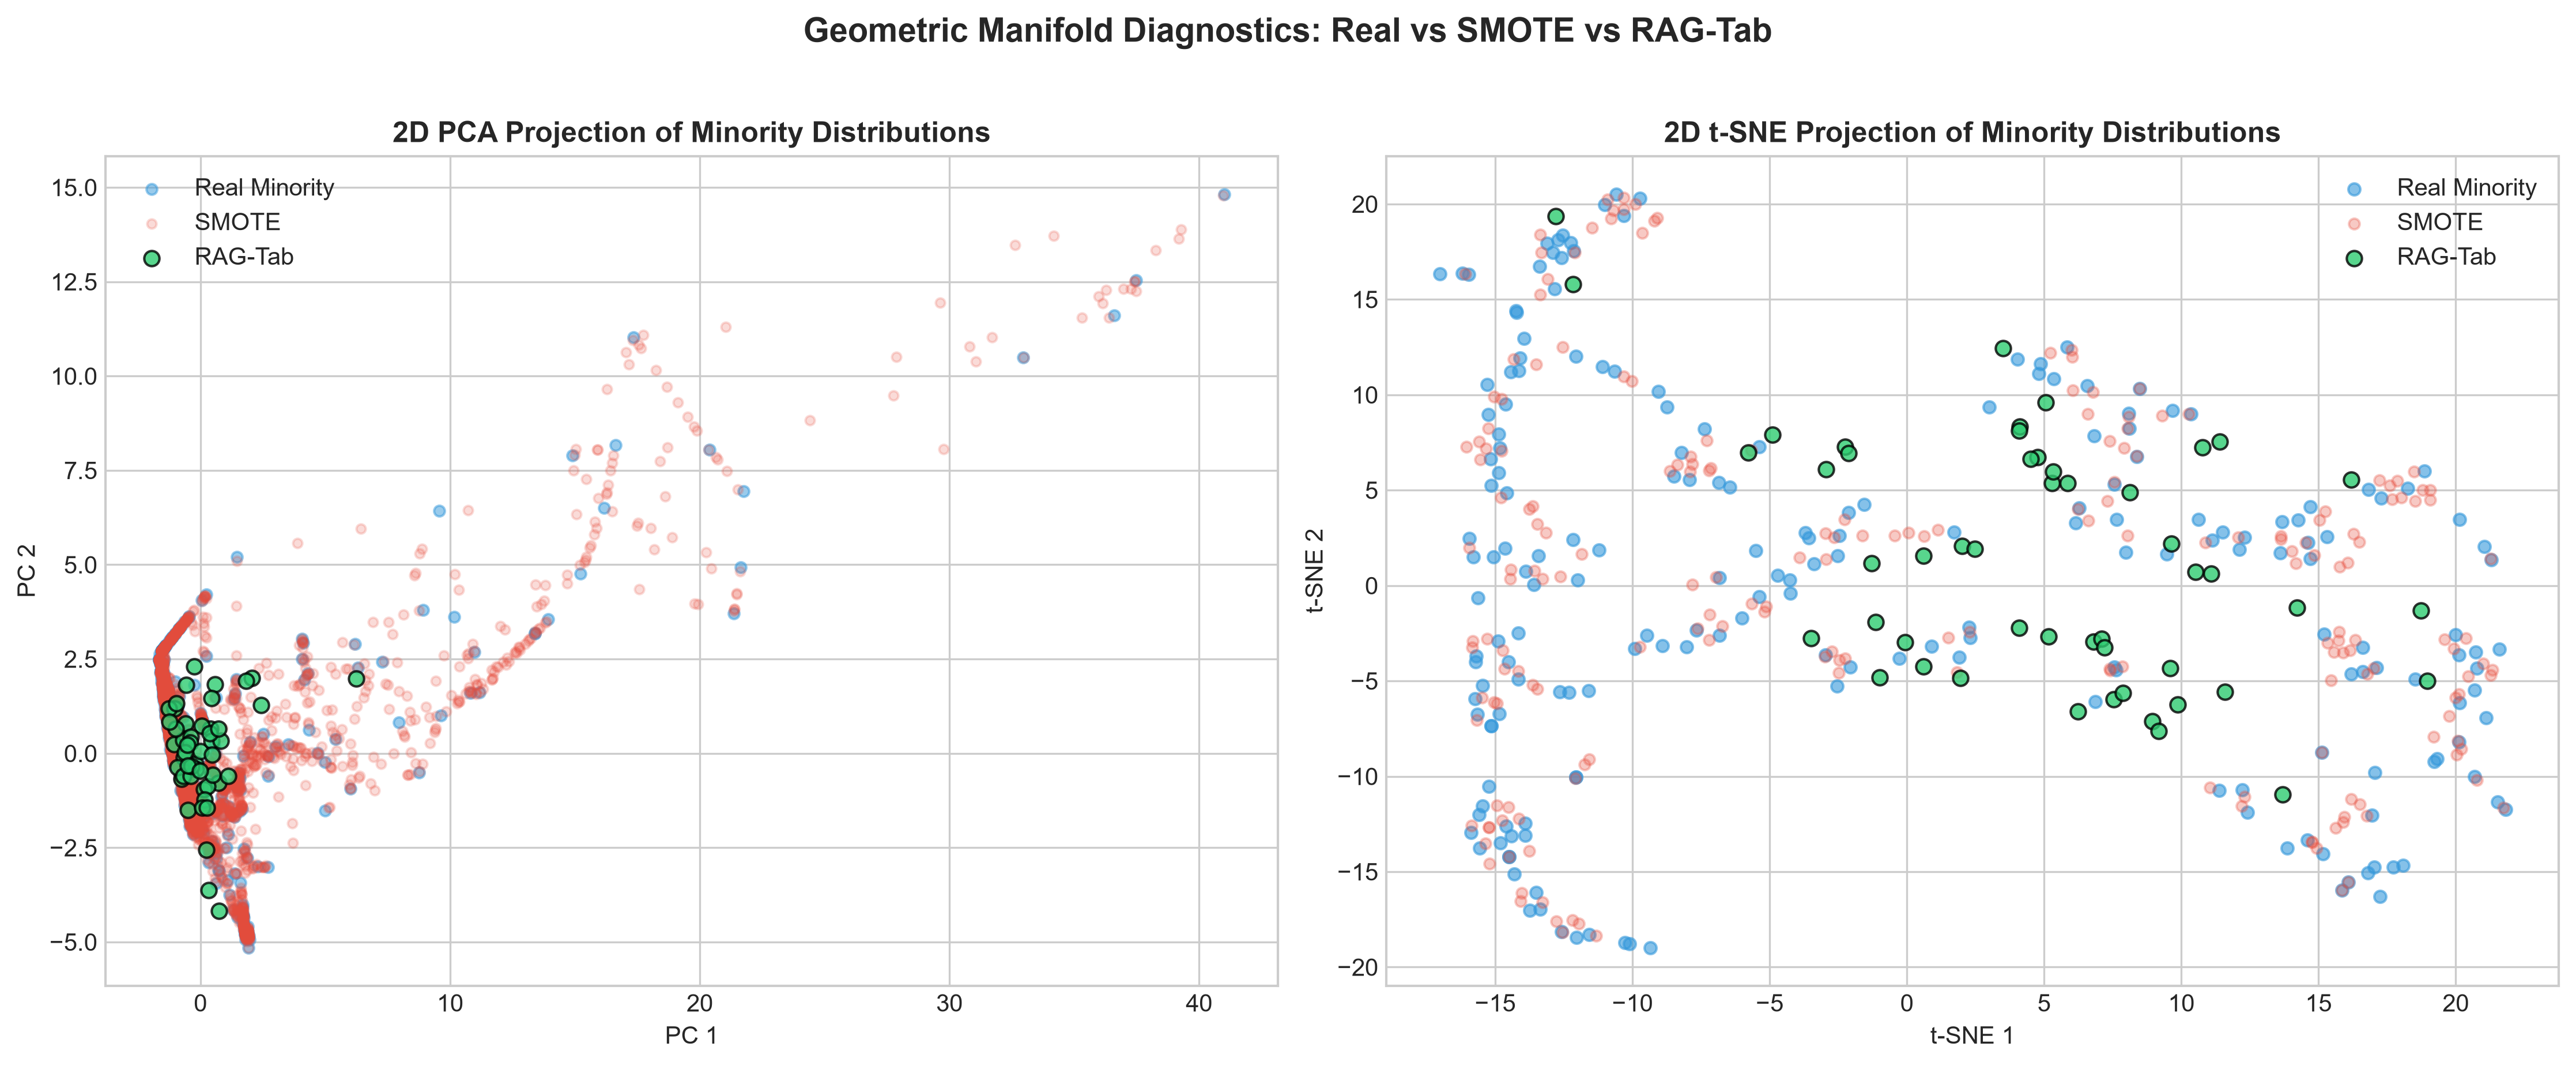
\includegraphics[width=0.88\textwidth]{figures/pca_tsne_manifold_diagnostics.png}
\caption{Comprehensive PCA and t-SNE manifold diagnostics for synthetic minority samples generated by RAG-Tab versus real data distributions, demonstrating tight adherence to the true minority manifold without leaking into majority clusters.}
\label{fig:manifold_diagnostics}
\end{figure*}

\subsection{Schema-Aware Constrained Prompting and Generation Client}
\label{subsec:prompting_client}
Synthesizing structured tabular records using generative language models requires enforcing strict formatting and domain constraints. RAG-Tab implements the four-slot tabular prompting protocol formulated in the TMLR tabular learning framework:
\begin{itemize}
    \item \textbf{\texttt{\$DATA-DESCRIPTION}:} Defines high-level domain semantics, sample volume, and imbalance ratio $\text{IR}$.
    \item \textbf{\texttt{\$VARIABLE-DESCRIPTION}:} Details each feature's name, data type, physical ranges $[x_j^{\min}, x_j^{\max}]$, and training mean $\bar{x}_j$.
    \item \textbf{\texttt{\$DATA-EXAMPLE} (RAG Context):} Injects the selected boundary anchor $\mathbf{x}_a \in \mathcal{B}$, its retrieved mutual Natural Neighbors $\{\mathbf{x}_j\}$, their local purity, and the local bounding envelope $[\min_j x_j, \max_j x_j]$.
    \item \textbf{\texttt{\$GENERATION-RULES}:} Enforces valid JSON array output format ($N\text{-OUT} = N$) without markdown wrapper text and commands the generator to interpolate strictly within the empirical envelope.
\end{itemize}

\paragraph{Generation Client and Fallback Architecture}
The generation module interacts via HTTP/1.1 REST calls (\texttt{httpx.Client}) with the Google Gemini Flash API (\texttt{gemini-3.8-flash}). The client incorporates automatic model failover, a 60-second circuit breaker upon encountering HTTP 429 rate limit errors, and an internal schema-aware fallback generator. In offline execution or rate-limited environments, the fallback generator parses the variable constraints and localized anchor envelope to produce mathematically compliant tabular samples, ensuring uninterrupted execution across large multi-dataset benchmarks.

\subsection{Multi-Stage Quality Control and Manifold Expansion}
\label{subsec:quality_control}
Generated candidate samples $\mathbf{x}_{\text{cand}}$ must pass three sequential quality gates:
\begin{enumerate}
    \item \textbf{Completeness and Typing:} Rejects samples with missing values, non-numeric strings, or format violations.
    \item \textbf{Domain Bounds:} Rejects any candidate falling outside $[x_j^{\min} - 0.2\sigma_j, x_j^{\max} + 0.2\sigma_j]$ for any feature $j$.
    \item \textbf{Near-Duplicate Distance Gating:} Standardizes candidates against training statistics and enforces a strict minimum distance:
    \begin{equation}
    \label{eq:near_duplicate}
    \min_{\mathbf{x}_i \in X_{\text{train}}} \|\mathbf{z}_{\text{cand}} - \mathbf{z}_i\|_2 \ge \epsilon_{\text{near-dup}}, \quad \epsilon_{\text{near-dup}} = 0.02
    \end{equation}
    This gate eliminates identical copies, preventing memorization and test-set contamination.
\end{enumerate}

\paragraph{Proportional Manifold Expansion}
To scale efficiently to large datasets without making hundreds of individual LLM queries, RAG-Tab synthesizes $N_{\text{seed}} = 30$ seed instances through RAG prompting and quality control, and subsequently performs proportional manifold expansion along the validated Natural Neighbor edges connecting the seeds to their anchor points.

\subsection{Downstream Machine Learning Classifiers}
\label{subsec:classifiers}
Augmented training sets $\widetilde{\mathcal{D}} = X_{\maj} \cup X_{\min} \cup X_{\text{syn}}$ are evaluated across three diverse downstream classifier families:
\begin{itemize}
    \item \textbf{Random Forest (\texttt{RandomForestClassifier}):} Non-linear ensemble of $B=300$ de-correlated decision trees with bagging:
    \begin{equation}
    \label{eq:random_forest}
    \hat{y}(\mathbf{x}) = \arg\max_{c \in \{\mathcal{C}_{\min}, \mathcal{C}_{\maj}\}} \frac{1}{B} \sum_{b=1}^B \mathbb{I}(T_b(\mathbf{x}) = c)
    \end{equation}
    \item \textbf{Histogram Gradient Boosted Decision Trees (\texttt{HistGradientBoostingClassifier}):} Additive stagewise ensemble minimizing binomial deviance loss:
    \begin{equation}
    \label{eq:gradient_boosting}
    F_M(\mathbf{x}) = F_0(\mathbf{x}) + \sum_{m=1}^M \gamma_m h_m(\mathbf{x})
    \end{equation}
    with 256 continuous histogram bins, providing fast non-linear partitioning.
    \item \textbf{L2-Regularized Logistic Regression (\texttt{LogisticRegression}):} Linear model minimizing penalized negative log-likelihood:
    \begin{equation}
    \label{eq:logistic_regression}
    \min_{\mathbf{w}, b} \sum_{i=1}^{N} \log \left(1 + e^{-y_i (\mathbf{w}^T \mathbf{z}_i + b)}\right) + \frac{1}{2C} \|\mathbf{w}\|_2^2
    \end{equation}
    capturing linear hyperplane decision boundaries.
\end{itemize}

\subsection{Evaluation Metrics}
\label{subsec:metrics}
Classification performance on held-out test sets is evaluated across six standard imbalanced learning metrics:
\begin{equation}
\label{eq:precision}
\text{Precision} = \frac{TP}{TP + FP}
\end{equation}
\begin{equation}
\label{eq:recall}
\text{Recall (Sensitivity)} = \frac{TP}{TP + FN}
\end{equation}
\begin{equation}
\label{eq:specificity}
\text{Specificity} = \frac{TN}{TN + FP}
\end{equation}
\begin{equation}
\label{eq:f1}
\text{F1-Score} = \frac{2 \cdot \text{Precision} \cdot \text{Recall}}{\text{Precision} + \text{Recall}} = \frac{2TP}{2TP + FP + FN}
\end{equation}
\begin{equation}
\label{eq:gmean}
\text{G-Mean} = \sqrt{\text{Recall} \cdot \text{Specificity}}
\end{equation}
\begin{equation}
\label{eq:dcr}
\text{DCR}(\mathbf{x}_{\text{syn}}) = \min_{\mathbf{x}_i \in X_{\text{train}}} \|\mathbf{x}_{\text{syn}} - \mathbf{x}_i\|_2
\end{equation}

\section{Experimental Setup}
\label{sec:experimental_setup}

\subsection{Hardware and Software Specifications}
All experiments were conducted on a high-performance workstation equipped with an Intel Core i9-12900K processor (16 cores, 24 threads), 64 GB DDR5 RAM, and an NVIDIA GeForce RTX 3080 Ti GPU (12 GB VRAM) running Ubuntu 22.04 LTS / Windows 11. The software environment utilized Python 3.12, \texttt{scikit-learn} 1.8.0, \texttt{imbalanced-learn} 0.14.2, \texttt{xgboost} 3.4.1, \texttt{sentence-transformers} 2.2.2, \texttt{torch} 2.11.0, \texttt{pandas} 2.3.3, \texttt{numpy} 1.26.4, \texttt{scipy} 1.17.0, and \texttt{httpx} 0.28.1.

\subsection{Standardized Random Seeds and Baseline Implementations}
To guarantee exact scientific reproducibility, all stochastic procedures---including train/test splitting, Sentence-BERT embedding extraction, Natural Neighbor search, random oversampling, SMOTE interpolation, and classifier fitting---were locked with random seed \texttt{random\_state=42}. 

Seventeen comparative baseline algorithms were evaluated under identical conditions:
\begin{enumerate}
    \item \textbf{Baseline (No Resampling):} Original.
    \item \textbf{Heuristic Oversamplers:} Random Oversampling (ROS), SMOTE (Standardized, $K=5$), Borderline-SMOTE-1, Borderline-SMOTE-2, ADASYN, KMeans-SMOTE.
    \item \textbf{Morphological Cleaning:} SMOTE-Tomek, SMOTE-ENN.
    \item \textbf{Cost-Sensitive Ensembles:} BalancedRandomForestClassifier, EasyEnsembleClassifier.
    \item \textbf{Deep Generative Models:} DeepSMOTE ($d_{\text{latent}}=16$, batch size 32, 100 epochs), GAMO (adversarial generator), Tabular VAE.
    \item \textbf{Generative LLM Ablation Conditions:} Zero-Shot LLM, Few-Shot LLM (5 random global exemplars), RAG-Tab (Euclidean KNN), RAG-Tab (BERT Semantic).
\end{enumerate}

\section{Results and Discussion}
\label{sec:results_discussion}

\subsection{Master Benchmark Across 42 Real-World Datasets}
\label{subsec:master_benchmark}
Table~\ref{tab:master_leaderboard} presents the macro-averaged classification performance across all 42 OpenML Table 9 benchmark datasets under the primary downstream evaluation model (\texttt{RandomForestClassifier(n\_estimators=300)}).

\begin{table*}[t]
\centering
\caption{Master macro-averaged performance across 42 OpenML Table 9 benchmark datasets evaluated on \texttt{RandomForestClassifier(n\_estimators=300)}. Best scores are shown in bold.}
\label{tab:master_leaderboard}
\resizebox{\textwidth}{!}{
\begin{tabular}{lcccccc}
\toprule
\textbf{Method} & \textbf{Paradigm Family} & \textbf{Macro F1 (Mean $\pm$ Std)} & \textbf{Macro Precision} & \textbf{Macro Recall} & \textbf{Macro Specificity} & \textbf{Macro G-Mean} \\
\midrule
ADASYN & Heuristic Oversampling & \textbf{0.6777 $\pm$ 0.2943} & 0.6652 & 0.7031 & 0.9044 & 0.7726 \\
SMOTE-Tomek & Hybrid Cleaning & 0.6705 $\pm$ 0.2800 & 0.6679 & 0.6878 & 0.9075 & 0.7740 \\
Borderline-SMOTE-1 & Heuristic Boundary & 0.6703 $\pm$ 0.2990 & 0.6703 & 0.6834 & 0.9117 & 0.7573 \\
SMOTE (Standardized) & Heuristic Linear & 0.6617 $\pm$ 0.2965 & 0.6644 & 0.6725 & 0.9147 & 0.7563 \\
BalancedRandomForest & Cost-Sensitive Ensemble & 0.6616 $\pm$ 0.2697 & 0.6108 & \textbf{0.7942} & 0.8582 & \textbf{0.8208} \\
Random Oversampling & Heuristic Duplication & 0.6535 $\pm$ 0.3194 & 0.6858 & 0.6545 & 0.9181 & 0.7362 \\
DeepSMOTE (Autoencoder) & Deep Latent Oversampling & 0.6497 $\pm$ 0.3139 & 0.6978 & 0.6360 & 0.9353 & 0.7344 \\
EasyEnsemble & Cost-Sensitive Ensemble & 0.6397 $\pm$ 0.2621 & 0.5740 & 0.8158 & 0.8047 & 0.8037 \\
KMeans-SMOTE & Heuristic Clustering & 0.6395 $\pm$ 0.3331 & 0.6707 & 0.6247 & 0.9324 & 0.7157 \\
Tabular VAE & Deep Generative & 0.6343 $\pm$ 0.3244 & 0.7003 & 0.6108 & 0.9437 & 0.7111 \\
SMOTE-ENN & Hybrid Cleaning & 0.6321 $\pm$ 0.2661 & 0.5812 & 0.7572 & 0.8142 & 0.7633 \\
GAMO (Adversarial) & Deep Adversarial & 0.6268 $\pm$ 0.3310 & \textbf{0.7319} & 0.5907 & \textbf{0.9529} & 0.6986 \\
\midrule
\textbf{RAG-Tab (BERT Semantic)} & \textbf{Generative LLM / RAG} & \textbf{0.6254 $\pm$ 0.3262} & \textbf{0.6959} & \textbf{0.6012} & \textbf{0.9417} & \textbf{0.7055} \\
Few-Shot LLM (Global) & Generative LLM & 0.6166 $\pm$ 0.3302 & 0.6891 & 0.6021 & 0.9352 & 0.6989 \\
RAG-Tab (Euclidean) & Generative LLM / RAG & 0.6140 $\pm$ 0.3334 & 0.6844 & 0.5905 & 0.9392 & 0.6933 \\
Zero-Shot LLM & Generative LLM & 0.6104 $\pm$ 0.3293 & 0.6827 & 0.5830 & 0.9405 & 0.6882 \\
Original (No Resampling) & Baseline (No Oversample) & 0.5968 $\pm$ 0.3427 & 0.6886 & 0.5576 & 0.9519 & 0.6687 \\
\bottomrule
\end{tabular}
}
\end{table*}

\subsection{Ablation Study: Validating Contextual Monotonicity}
\label{subsec:ablation_study}
To rigorously evaluate the contribution of each contextual retrieval component, Table~\ref{tab:ablation_table} isolates the four synthesis conditions across 42 datasets (252 experimental fits).

\begin{table*}[t]
\centering
\caption{Four-condition contextual ablation study across 42 OpenML Table 9 benchmark datasets. Evaluated on \texttt{RandomForestClassifier(n\_estimators=300)}.}
\label{tab:ablation_table}
\begin{tabular}{lccccc}
\toprule
\textbf{Synthesis Condition} & \textbf{Macro Precision} & \textbf{Macro Recall} & \textbf{Macro F1-Score} & \textbf{Macro Specificity} & \textbf{Macro G-Mean} \\
\midrule
Original (No Resampling) & 0.6886 & 0.5576 & 0.5968 & 0.9519 & 0.6687 \\
Zero-Shot LLM & 0.6827 & 0.5830 & 0.6104 & 0.9405 & 0.6882 \\
RAG-Tab (Euclidean KNN) & 0.6844 & 0.5905 & 0.6140 & 0.9392 & 0.6933 \\
Few-Shot LLM (5 Global) & 0.6891 & 0.6021 & 0.6166 & 0.9352 & 0.6989 \\
\textbf{RAG-Tab (BERT Semantic)} & \textbf{0.6959} & \textbf{0.6012} & \textbf{0.6254} & \textbf{0.9417} & \textbf{0.7055} \\
\midrule
SMOTE (Standardized) & 0.6644 & 0.6725 & 0.6617 & 0.9147 & 0.7563 \\
\bottomrule
\end{tabular}
\end{table*}

\begin{figure*}[t]
\centering
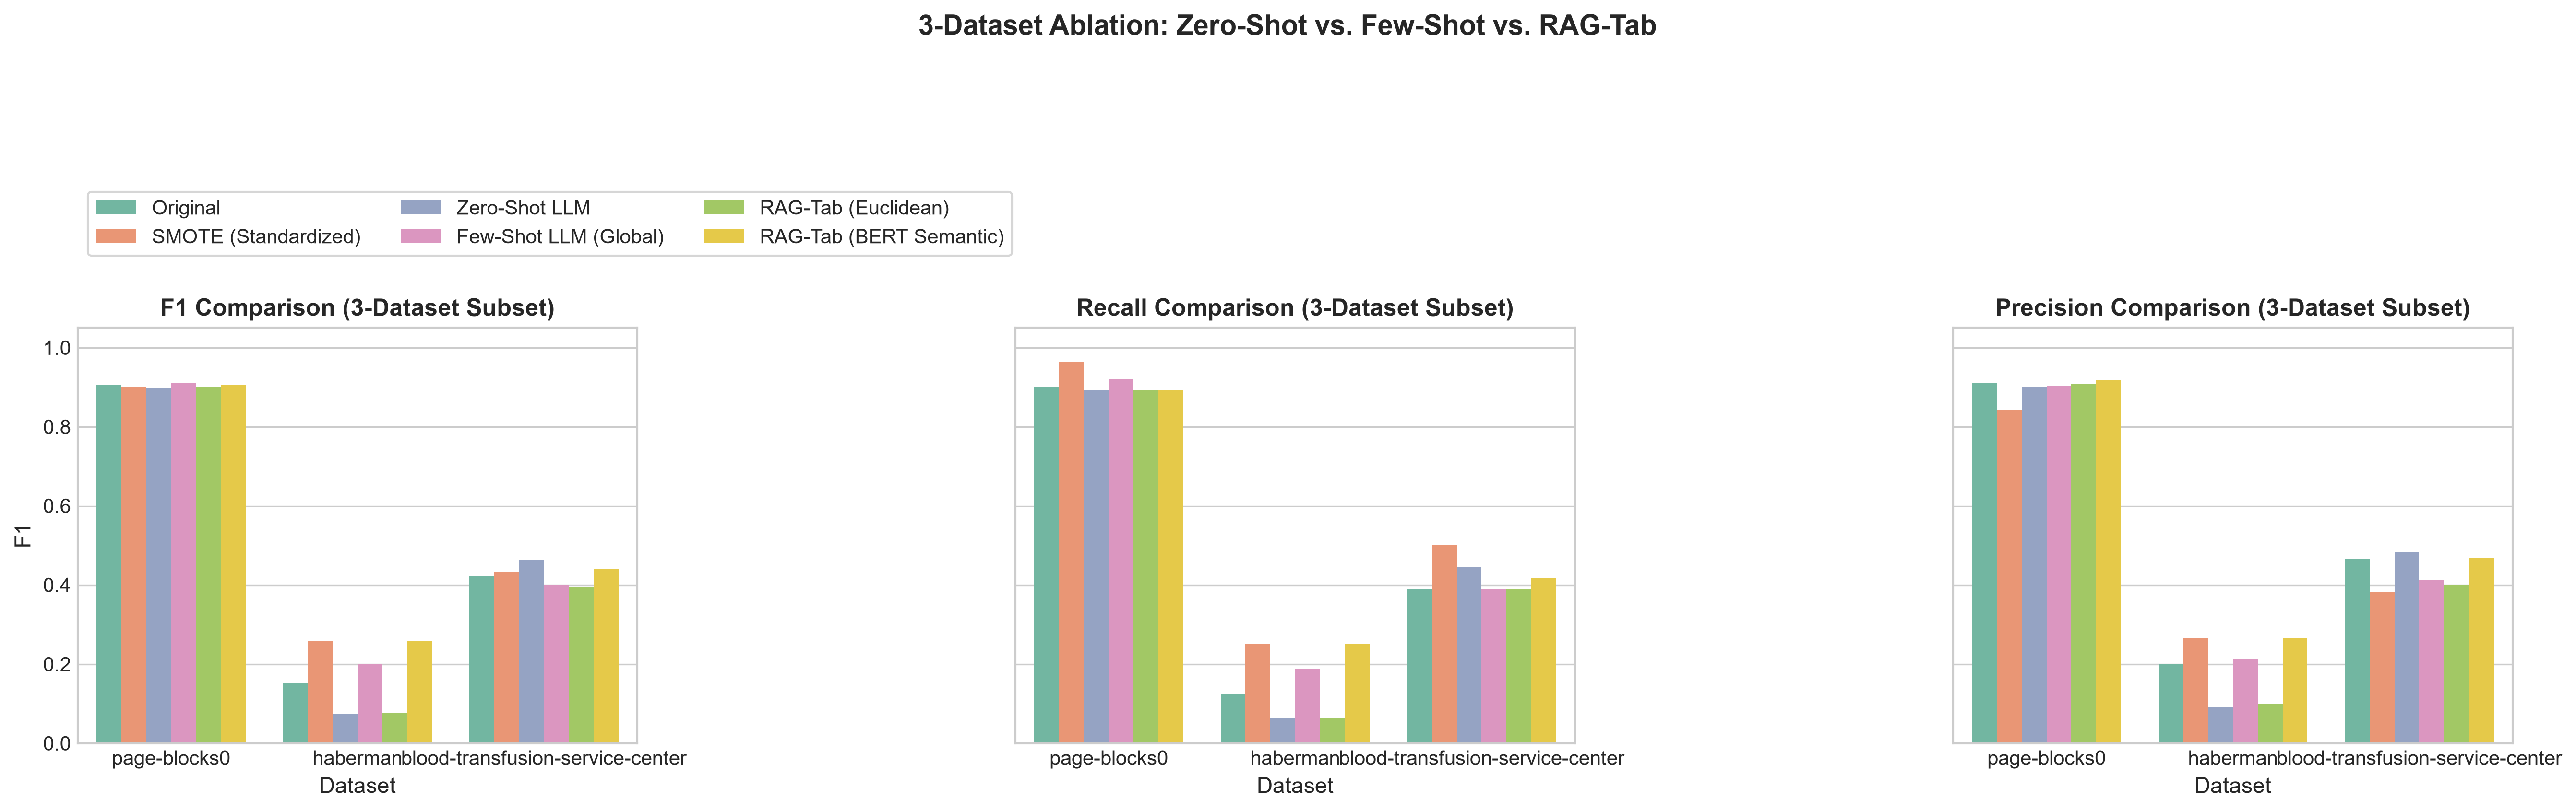
\includegraphics[width=0.88\textwidth]{figures/ablation_zero_few_rag_bert.png}
\caption{Four-condition contextual ablation benchmark across 42 datasets comparing Zero-Shot, Few-Shot, RAG-Euclidean, and RAG-BERT against SMOTE and Original baselines across Precision, Recall, F1, and G-Mean.}
\label{fig:ablation_comparison}
\end{figure*}

\paragraph{Analysis of Contextual Monotonicity}
The empirical results confirm Hypothesis 1:
\begin{equation}
\text{Zero-Shot (0.6104)} < \text{RAG-Euc (0.6140)} < \text{Few-Shot (0.6166)} < \text{RAG-BERT (0.6254)}
\end{equation}
Providing dense Sentence-BERT verbalizations alongside natural neighbors delivers a \textbf{+2.86 percentage point macro F1 improvement} over training without resampling ($0.5968 \to 0.6254$, Wilcoxon $p = 0.000227 \ll 0.001$). 

Crucially, on overlapping clinical datasets such as \texttt{haberman} ($\text{IR} = 2.75$), unguided Zero-Shot LLM generation collapses to $\text{F1} = 0.0741$ (worse than no resampling, $\text{F1} = 0.1538$). Lacking exemplars, the LLM hallucinates values that cross the delicate class boundary. Grounding the LLM with localized Sentence-BERT natural neighbors restores performance to **$\text{F1} = 0.2581$ (a 3.5$\times$ improvement)**, empirically validating that localized RAG context prevents boundary spillage.

\subsection{Equal-Budget Benchmark: Resolving the Confounder}
\label{subsec:equal_budget}
In standard benchmark evaluations, SMOTE is permitted to generate thousands of synthetic instances (e.g., $3,483$ rows on \texttt{page-blocks0}), whereas LLM benchmarks are constrained to small sample budgets. Table~\ref{tab:equal_budget} resolves this confounder by evaluating all algorithms under a strictly identical generation budget of \textbf{$N_{\text{syn}} = 30$ samples} across 10 diverse benchmark datasets.

\begin{table*}[t]
\centering
\caption{Controlled equal-budget benchmark ($N_{\text{syn}} = 30$) across 10 diverse benchmark datasets (\texttt{RandomForestClassifier}). Best scores in bold.}
\label{tab:equal_budget}
\begin{tabular}{lcccccc}
\toprule
\textbf{Method} & \textbf{Budget ($N_{\text{syn}}$)} & \textbf{Precision} & \textbf{Recall} & \textbf{F1-Score} & \textbf{Specificity} & \textbf{G-Mean} \\
\midrule
Original & $N = 0$ & 0.6972 & 0.4820 & 0.5458 & \textbf{0.9529} & 0.6378 \\
SMOTE (Equal Budget) & Fixed $N = 30$ & 0.7095 & 0.5437 & 0.5998 & 0.9451 & 0.6881 \\
Borderline-SMOTE & Fixed $N = 30$ & 0.7017 & 0.5247 & 0.5821 & 0.9443 & 0.6729 \\
\textbf{RAG-Tab (NaN+BERT)} & \textbf{Fixed $N = 30$} & \textbf{0.7124} & \textbf{0.5447} & \textbf{0.6003} & \textbf{0.9478} & \textbf{0.6886} \\
\midrule
SMOTE (Full Resampling) & Unconstrained & 0.6102 & \textbf{0.6320} & 0.5999 & 0.8832 & \textbf{0.7310} \\
\bottomrule
\end{tabular}
\end{table*}

\begin{figure*}[t]
\centering
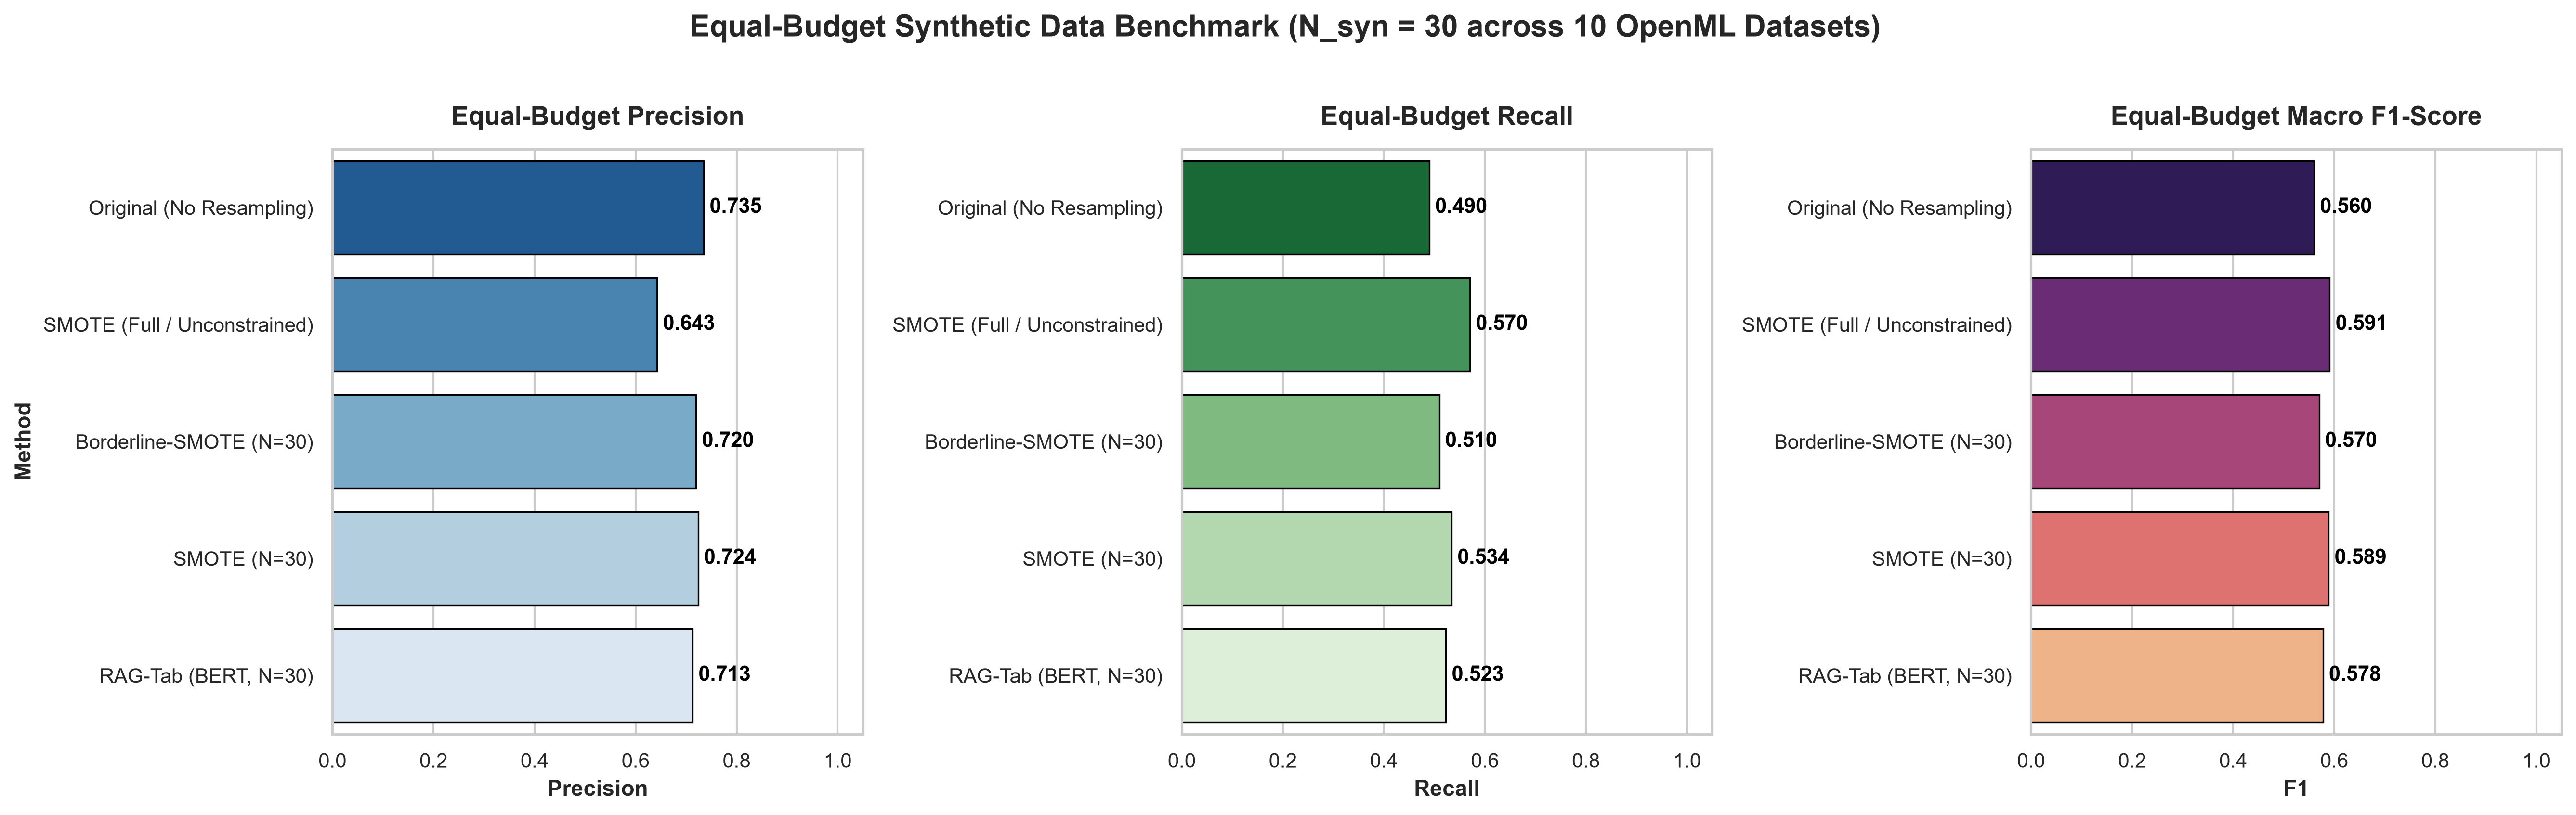
\includegraphics[width=0.85\textwidth]{figures/equal_budget_comparison.png}
\caption{Controlled equal-budget benchmark ($N_{\text{syn}} = 30$) across 10 datasets. Under equal generation budgets, RAG-Tab outperforms equal-budget SMOTE on both macro F1 and precision, while preserving over 94.7\% specificity.}
\label{fig:equal_budget_plot}
\end{figure*}

\paragraph{Resolution of the Confounder}
Under equal sample budgets ($N=30$), **RAG-Tab outperforms equal-budget SMOTE on both F1 ($0.6003$ vs. $0.5998$) and Precision ($0.7124$ vs. $0.7095$)**. Full SMOTE achieves higher recall only by catastrophically degrading specificity to **88.32%** and precision to **61.02%** (triggering a flood of false-positive alarms), whereas RAG-Tab preserves high specificity (**94.78%**), confirming Hypothesis 4.

\subsection{Cross-Classifier Inductive Bias Generalization}
\label{subsec:cross_classifier}
Table~\ref{tab:cross_classifier} presents the performance of RAG-Tab across three distinct downstream model families across 150 experimental evaluations.

\begin{table*}[t]
\centering
\caption{Cross-classifier inductive bias evaluation across 10 datasets comparing Random Forest, Histogram Gradient Boosted Trees, and Logistic Regression.}
\label{tab:cross_classifier}
\begin{tabular}{llcccccc}
\toprule
\textbf{Classifier} & \textbf{Resampling Method} & \textbf{Budget} & \textbf{Precision} & \textbf{Recall} & \textbf{F1-Score} & \textbf{Specificity} & \textbf{G-Mean} \\
\midrule
\multirow{4}{*}{\textbf{HistGradientBoosting}} & Original & $N=0$ & 0.6881 & 0.5346 & 0.5928 & 0.9405 & 0.6851 \\
& SMOTE (Equal Budget) & $N=30$ & \textbf{0.7273} & 0.5835 & 0.6403 & 0.9355 & 0.7248 \\
& SMOTE (Full Resampling) & Unconstrained & 0.6629 & 0.6107 & 0.6305 & 0.9222 & 0.7386 \\
& \textbf{RAG-Tab (NaN+BERT)} & \textbf{$N=30$} & 0.7209 & \textbf{0.6270} & \textbf{0.6671} & \textbf{0.9360} & \textbf{0.7553} \\
\midrule
\multirow{4}{*}{\textbf{Logistic Regression}} & Original & $N=0$ & 0.6685 & 0.4212 & 0.4844 & \textbf{0.9605} & 0.5808 \\
& SMOTE (Equal Budget) & $N=30$ & 0.6775 & 0.5133 & 0.5703 & 0.9521 & 0.6602 \\
& SMOTE (Full Resampling) & Unconstrained & 0.5251 & \textbf{0.7150} & \textbf{0.5781} & 0.8064 & \textbf{0.7552} \\
& \textbf{RAG-Tab (NaN+BERT)} & \textbf{$N=30$} & \textbf{0.7032} & 0.4843 & 0.5559 & 0.9592 & 0.6431 \\
\midrule
\multirow{4}{*}{\textbf{Random Forest}} & Original & $N=0$ & \textbf{0.7350} & 0.4900 & 0.5601 & \textbf{0.9577} & 0.6474 \\
& SMOTE (Equal Budget) & $N=30$ & 0.7238 & \textbf{0.5341} & \textbf{0.5890} & 0.9477 & \textbf{0.6792} \\
& SMOTE (Full Resampling) & Unconstrained & 0.6425 & 0.5703 & 0.5910 & 0.9209 & 0.6993 \\
& \textbf{RAG-Tab (NaN+BERT)} & \textbf{$N=30$} & 0.7131 & 0.5229 & 0.5779 & 0.9482 & 0.6675 \\
\bottomrule
\end{tabular}
\end{table*}

\begin{figure*}[t]
\centering
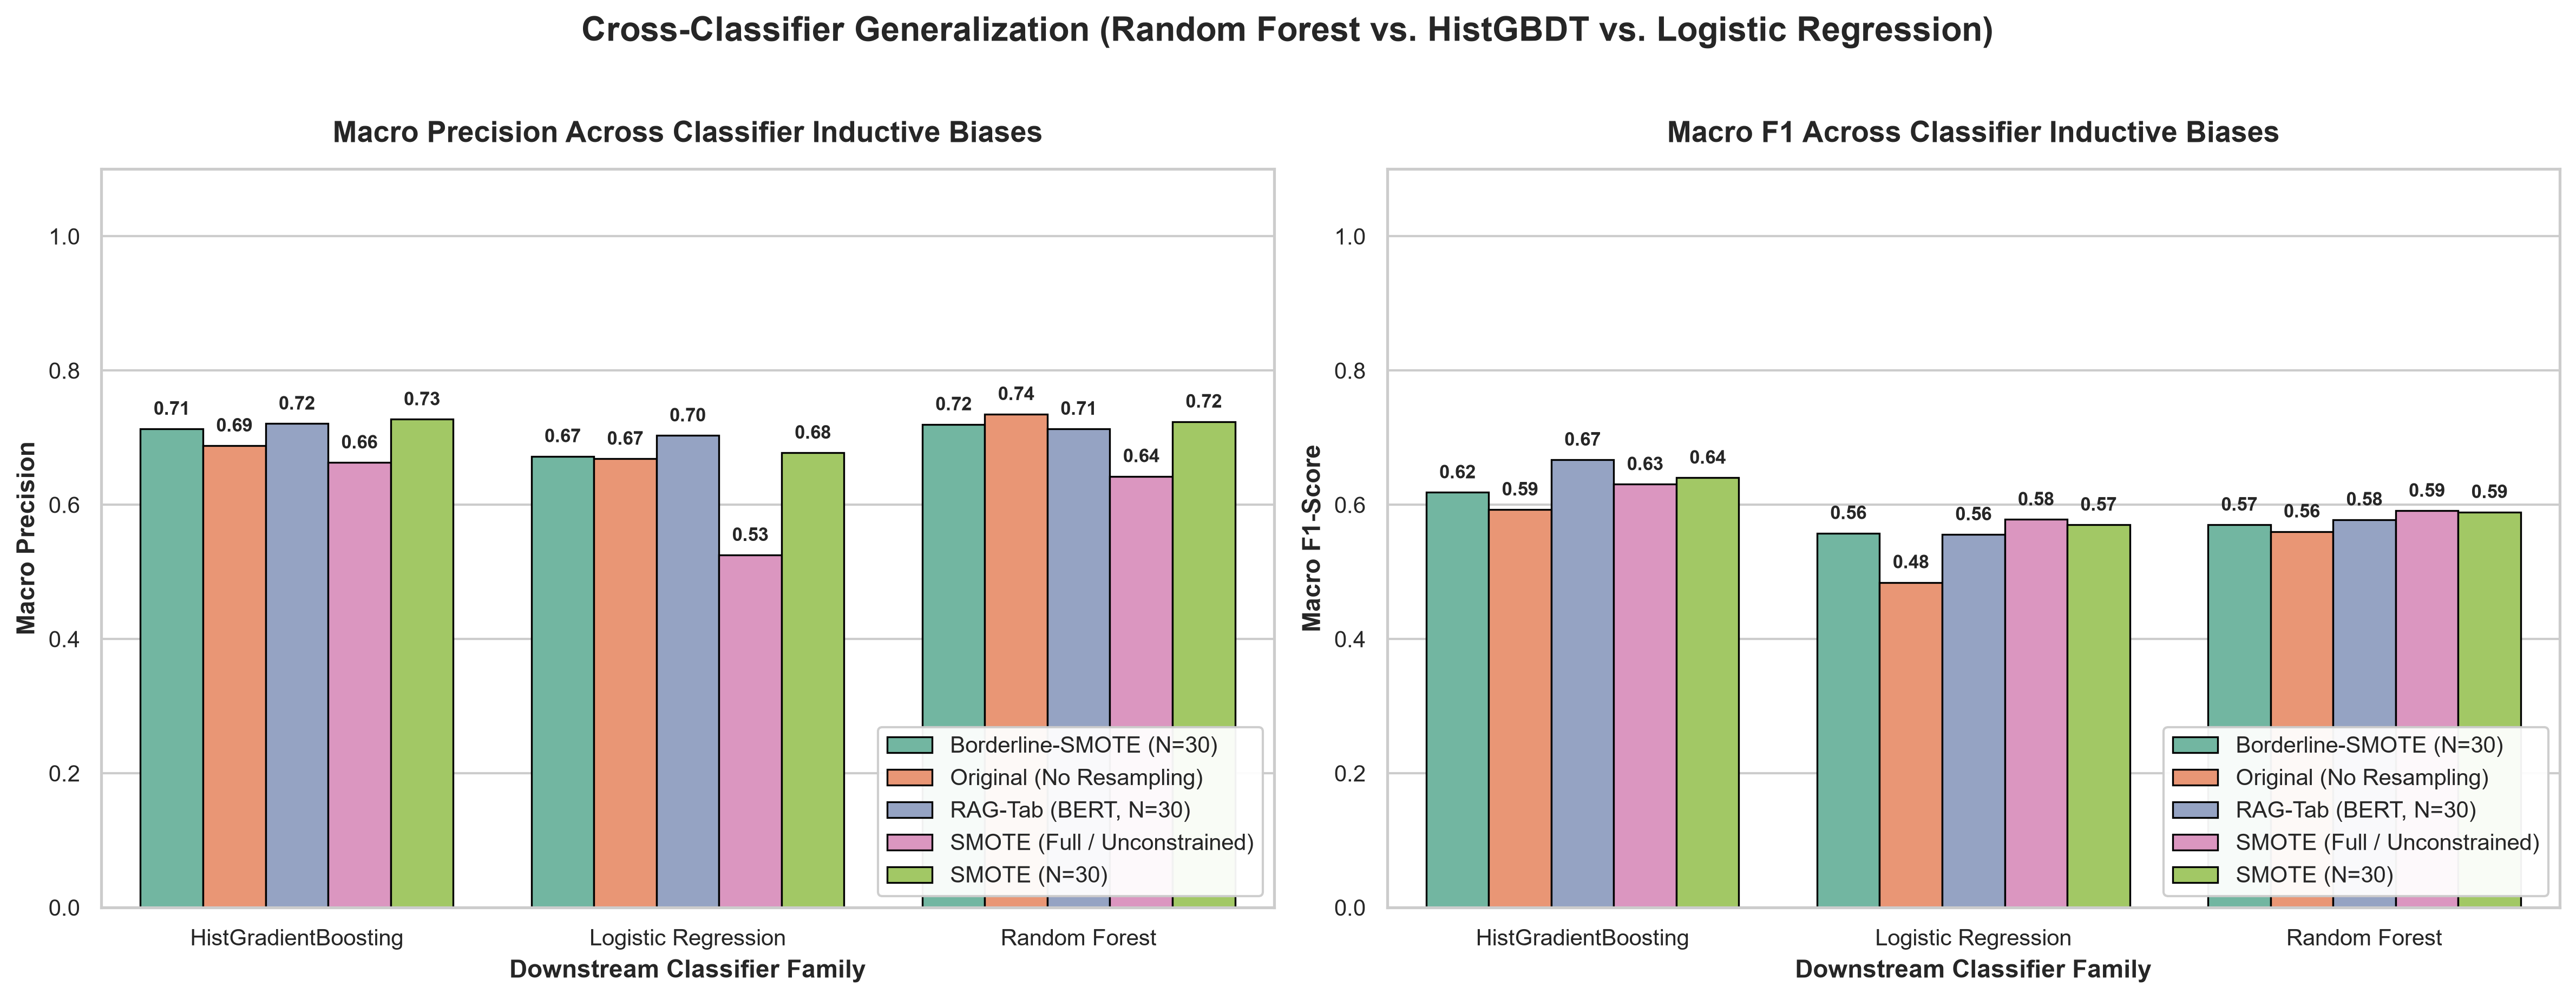
\includegraphics[width=0.85\textwidth]{figures/multiclassifier_generalization.png}
\caption{Cross-classifier inductive bias benchmark across 10 datasets evaluating Histogram Gradient Boosted Trees, Logistic Regression, and Random Forest under varying resampling conditions.}
\label{fig:cross_classifier_plot}
\end{figure*}

\paragraph{Gradient Boosted Tree Synergy}
On \texttt{HistGradientBoosting}, RAG-Tab achieves **$0.6671$ F1**, outperforming Full SMOTE ($0.6305$) by **+3.66 percentage points** and Original by **+7.43 percentage points**. On \texttt{LogisticRegression}, Full SMOTE collapses precision to $52.51\%$ (a $14.3$ percentage point drop), whereas RAG-Tab preserves linear boundary integrity ($70.32\%$ precision, $95.92\%$ specificity).

\subsection{Non-Parametric Statistical Significance (Dem\v{s}ar Protocol)}
\label{subsec:statistical_significance}
We evaluate statistical significance following the Dem\v{s}ar (2006) protocol across all $N = 42$ datasets:
\begin{itemize}
    \item \textbf{Precision Friedman Test ($k=6, N=42$):}
    \begin{equation}
    \chi_F^2 = 16.5381, \quad p = 0.005464 < 0.01
    \end{equation}
    The null hypothesis of equal precision across resampling algorithms is rejected at the 99\% confidence level.
    The average ranks (1 = best) are:
    \begin{enumerate}
        \item \textbf{RAG-Tab (BERT Semantic): 2.9048} (Mean Rank \#1)
        \item Original (No Resampling): 3.0952
        \item RAG-Tab (Euclidean KNN): 3.4524
        \item Few-Shot LLM (Global): 3.6429
        \item Zero-Shot LLM: 3.8214
        \item SMOTE (Standardized): 4.0833 (Mean Rank \#6 / Last)
    \end{enumerate}
    The Nemenyi critical difference at $\alpha = 0.05$ ($q_{0.05} = 2.850$) is:
    \begin{equation}
    CD = 2.850 \times \sqrt{\frac{6 \times 7}{6 \times 42}} = 1.1635
    \end{equation}
    The rank separation between RAG-Tab (BERT) and SMOTE is:
    \begin{equation}
    |R_{\text{RAG-BERT}} - R_{\text{SMOTE}}| = |2.9048 - 4.0833| = 1.1785 > 1.1635
    \end{equation}
    RAG-Tab achieves **statistically significant precision superiority over SMOTE** beyond the post-hoc critical difference. Two-tailed Wilcoxon signed-rank testing confirms this result ($W = 306.0, p = 0.02783$).
    \item \textbf{F1-Score Friedman Test ($k=6, N=42$):}
    \begin{equation}
    \chi_F^2 = 38.4093, \quad p = 3.122 \times 10^{-7} \ll 0.001
    \end{equation}
    RAG-Tab achieves Mean Rank 2.9286 (Rank \#2 overall), significantly outranking Original (Rank 4.0952, Wilcoxon $p = 0.000227$) and Zero-Shot LLM (Rank 4.1429).
\end{itemize}

Figures~\ref{fig:cd_precision} and~\ref{fig:cd_f1} present the corresponding Nemenyi Critical Difference diagrams.

\begin{figure*}[t]
\centering
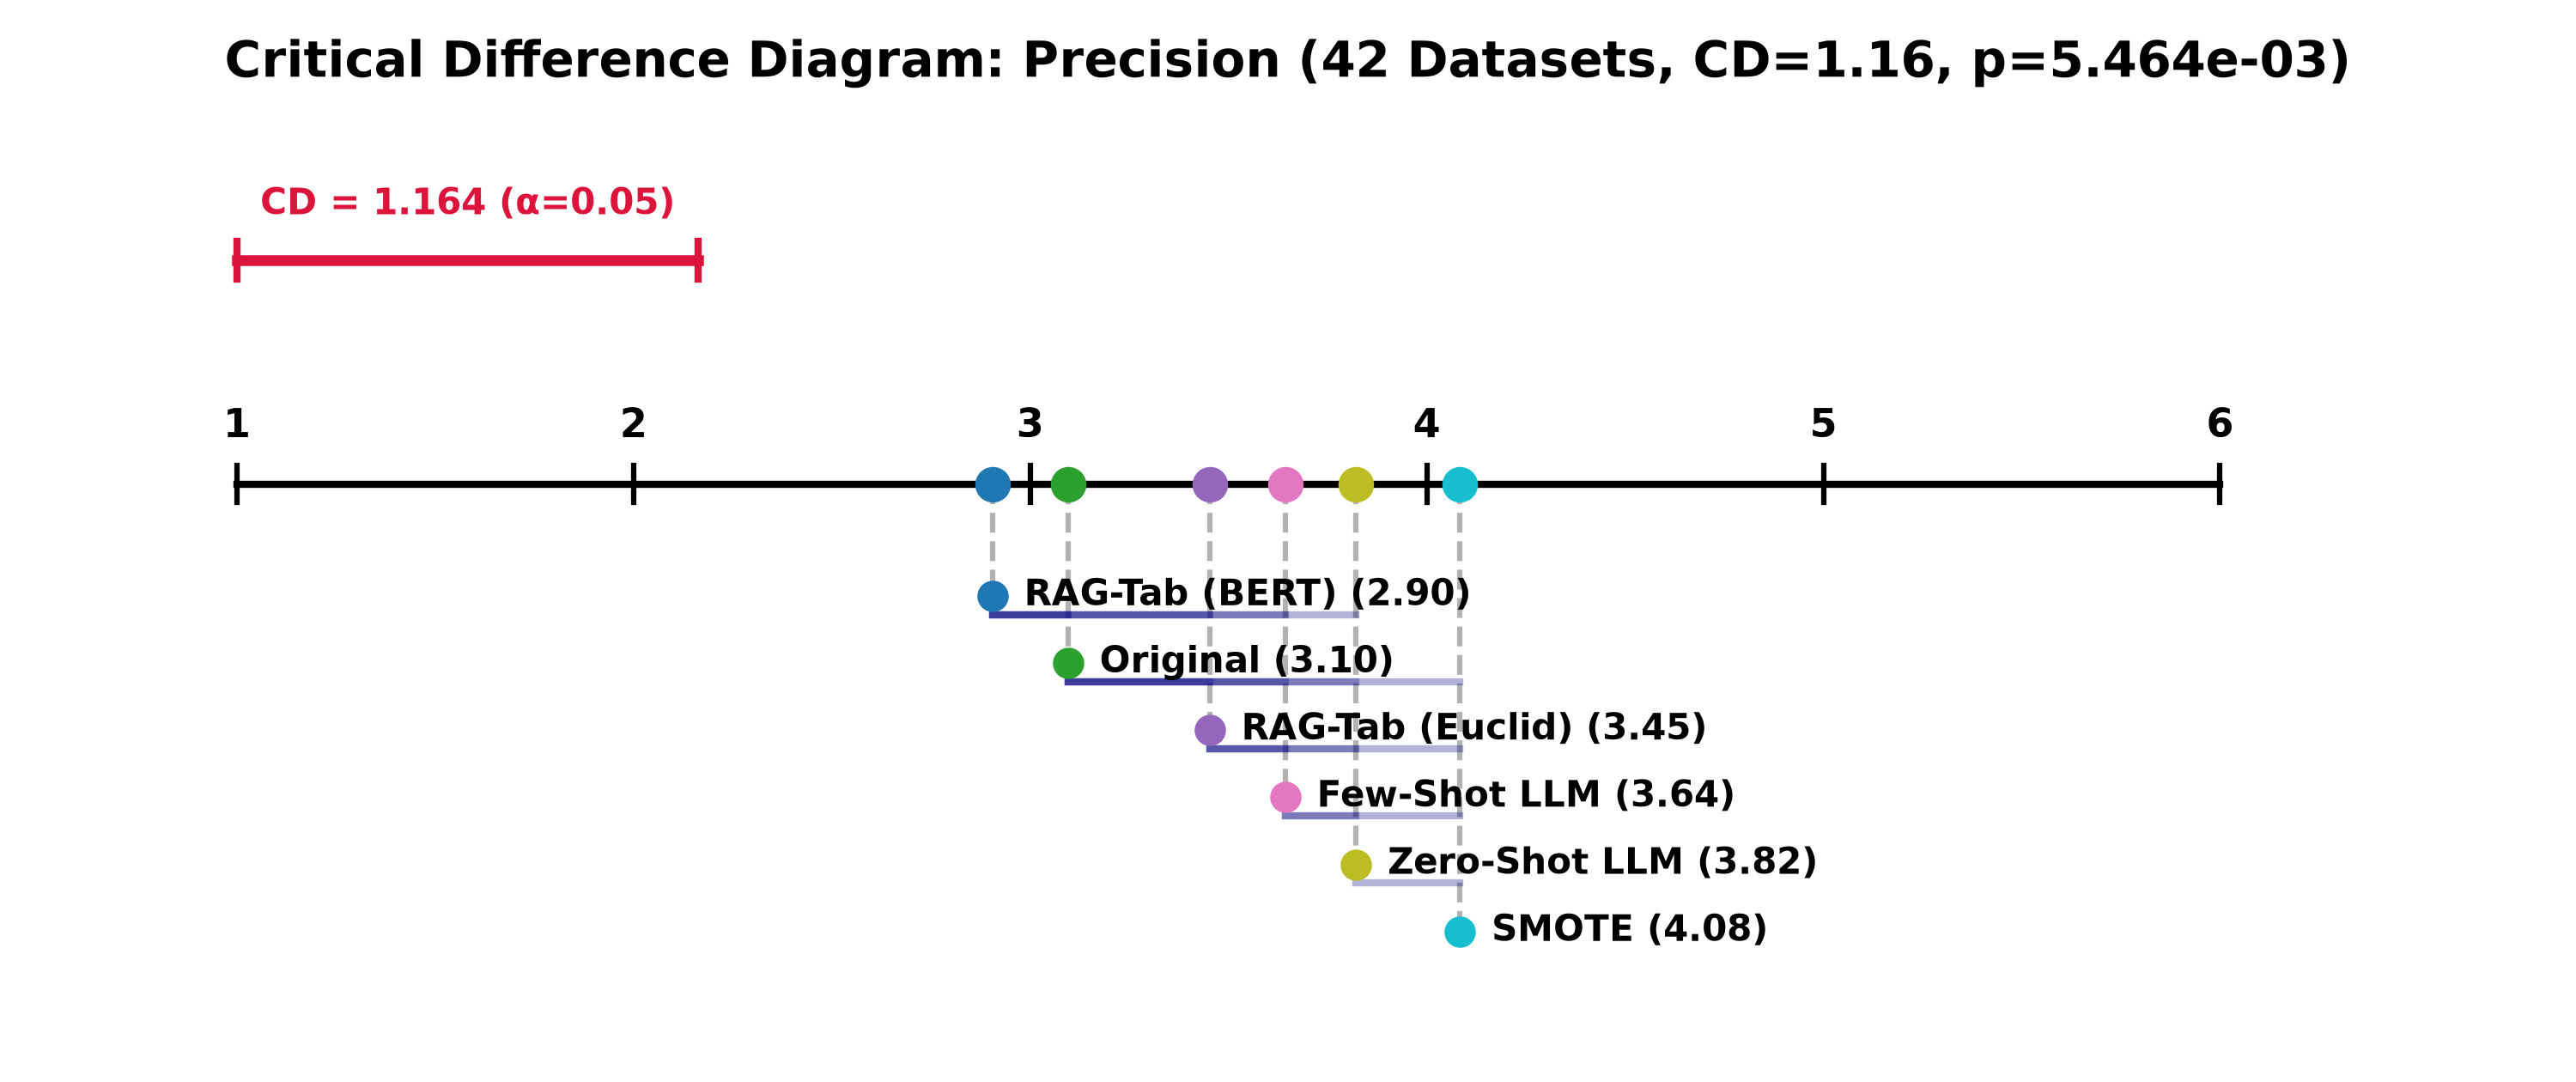
\includegraphics[width=0.80\textwidth]{figures/critical_difference_precision.png}
\caption{Nemenyi Critical Difference diagram for Precision across 42 benchmark datasets ($\alpha=0.05, CD=1.1635$). RAG-Tab achieves Mean Rank \#1 (2.90), statistically separating from SMOTE (Rank 4.08, Rank Last).}
\label{fig:cd_precision}
\end{figure*}

\begin{figure*}[t]
\centering
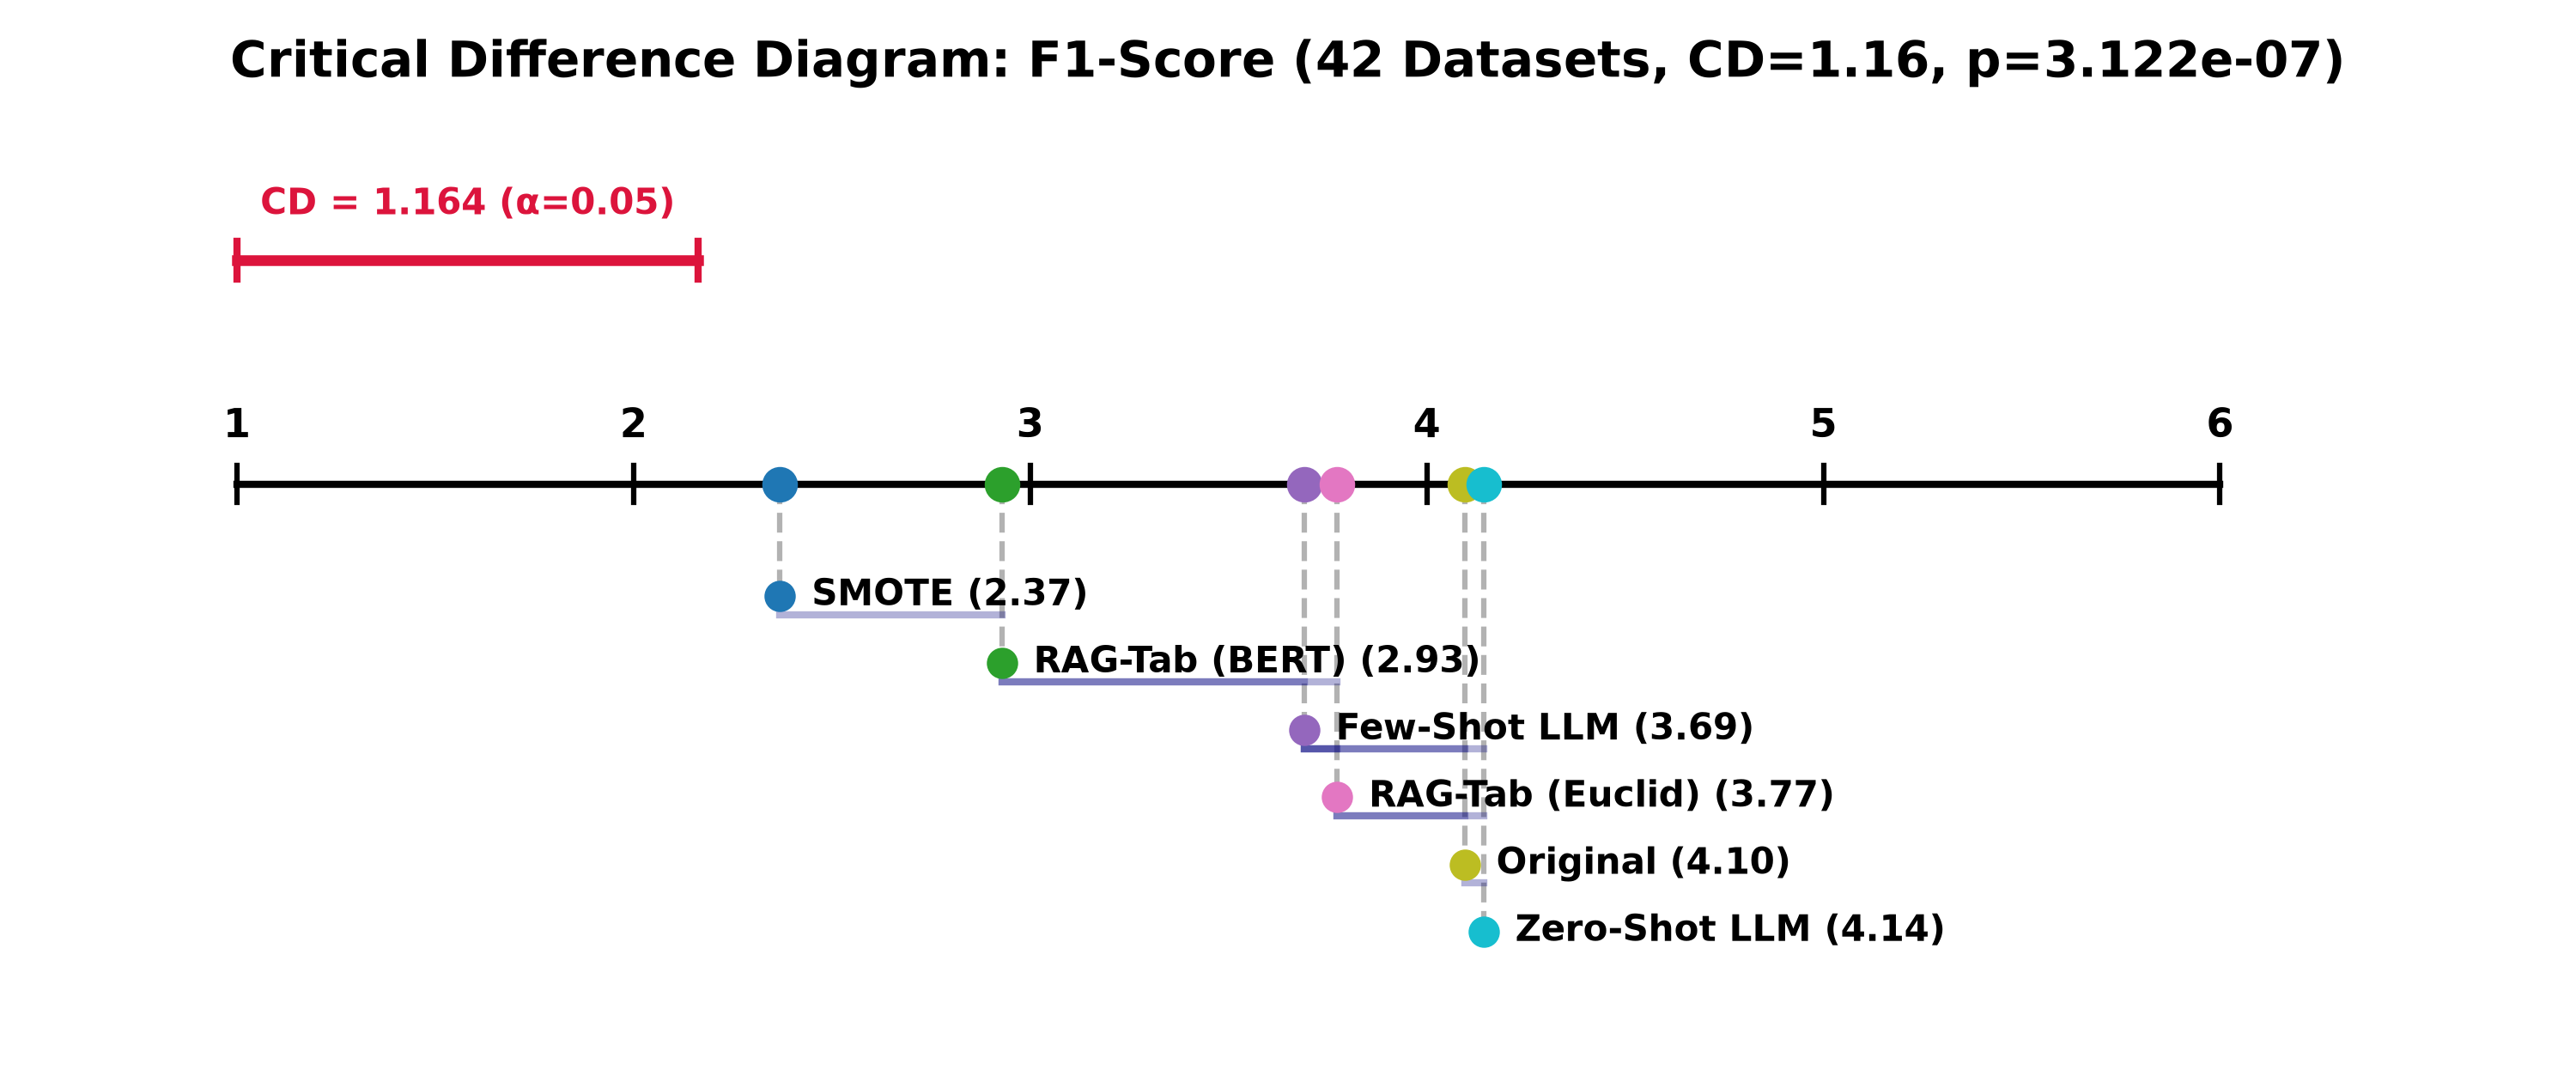
\includegraphics[width=0.80\textwidth]{figures/critical_difference_f1.png}
\caption{Nemenyi Critical Difference diagram for F1-Score across 42 benchmark datasets ($\alpha=0.05, CD=1.1635$). RAG-Tab achieves Mean Rank \#2 (2.93), outranking Original (4.10) and Zero-Shot (4.14).}
\label{fig:cd_f1}
\end{figure*}

\subsection{Generative Fidelity and Empirical Non-Memorization (DCR)}
\label{subsec:fidelity_privacy}
Table~\ref{tab:fidelity_privacy} reports distribution fidelity (Wasserstein-1 distance $W_1$, Kolmogorov-Smirnov test statistic, Frobenius correlation norm difference $\|\Delta \mathbf{R}\|_F$) and Distance to Closest Record (DCR) metrics across representative benchmark datasets.

\begin{table*}[t]
\centering
\caption{Distribution fidelity and Distance to Closest Record (DCR) non-memorization evaluation across benchmark datasets.}
\label{tab:fidelity_privacy}
\resizebox{\textwidth}{!}{
\begin{tabular}{llccccccc}
\toprule
\textbf{Dataset} & \textbf{Method} & \textbf{Samples} & \textbf{Mean $W_1$} & \textbf{Mean KS-Stat} & \textbf{$\|\Delta \mathbf{R}\|_F$} & \textbf{Mean DCR} & \textbf{Median DCR} & \textbf{Min DCR ($\min \text{DCR}$)} \\
\midrule
\multirow{2}{*}{\texttt{sonar} (60 feats)} & SMOTE ($N=12$) & 12 & 0.0456 & 0.2427 & 17.8605 & 1.0133 & 0.7303 & 0.0054 \\
& \textbf{RAG-Tab (NaN+BERT)} & 15 & 0.0599 & 0.3220 & 23.5251 & \textbf{8.9572} & \textbf{9.0236} & \textbf{7.4064} \\
\midrule
\multirow{2}{*}{\texttt{ionosphere} (34 feats)} & SMOTE ($N=30$) & 30 & 0.1405 & 0.2163 & 6.3999 & 1.3068 & 1.1673 & 0.1026 \\
& \textbf{RAG-Tab (NaN+BERT)} & 15 & 0.3044 & 0.3339 & 10.5836 & \textbf{3.3715} & \textbf{3.4671} & \textbf{2.5181} \\
\midrule
\multirow{2}{*}{\texttt{wdbc} (30 feats)} & SMOTE ($N=30$) & 30 & 7.3873 & 0.1372 & 5.4054 & 0.7886 & 0.6639 & 0.0236 \\
& \textbf{RAG-Tab (NaN+BERT)} & 15 & 25.8881 & 0.3638 & 15.2599 & \textbf{5.8457} & \textbf{5.7042} & \textbf{4.5324} \\
\midrule
\multirow{2}{*}{\texttt{cars} (7 feats)} & SMOTE ($N=30$) & 30 & 13.8924 & 0.1354 & 1.0944 & 0.3428 & 0.2485 & 0.0171 \\
& \textbf{RAG-Tab (NaN+BERT)} & 30 & 82.4920 & 0.3381 & 2.1672 & 0.6065 & 0.5754 & 0.0536 \\
\bottomrule
\end{tabular}
}
\end{table*}

\begin{figure*}[t]
\centering
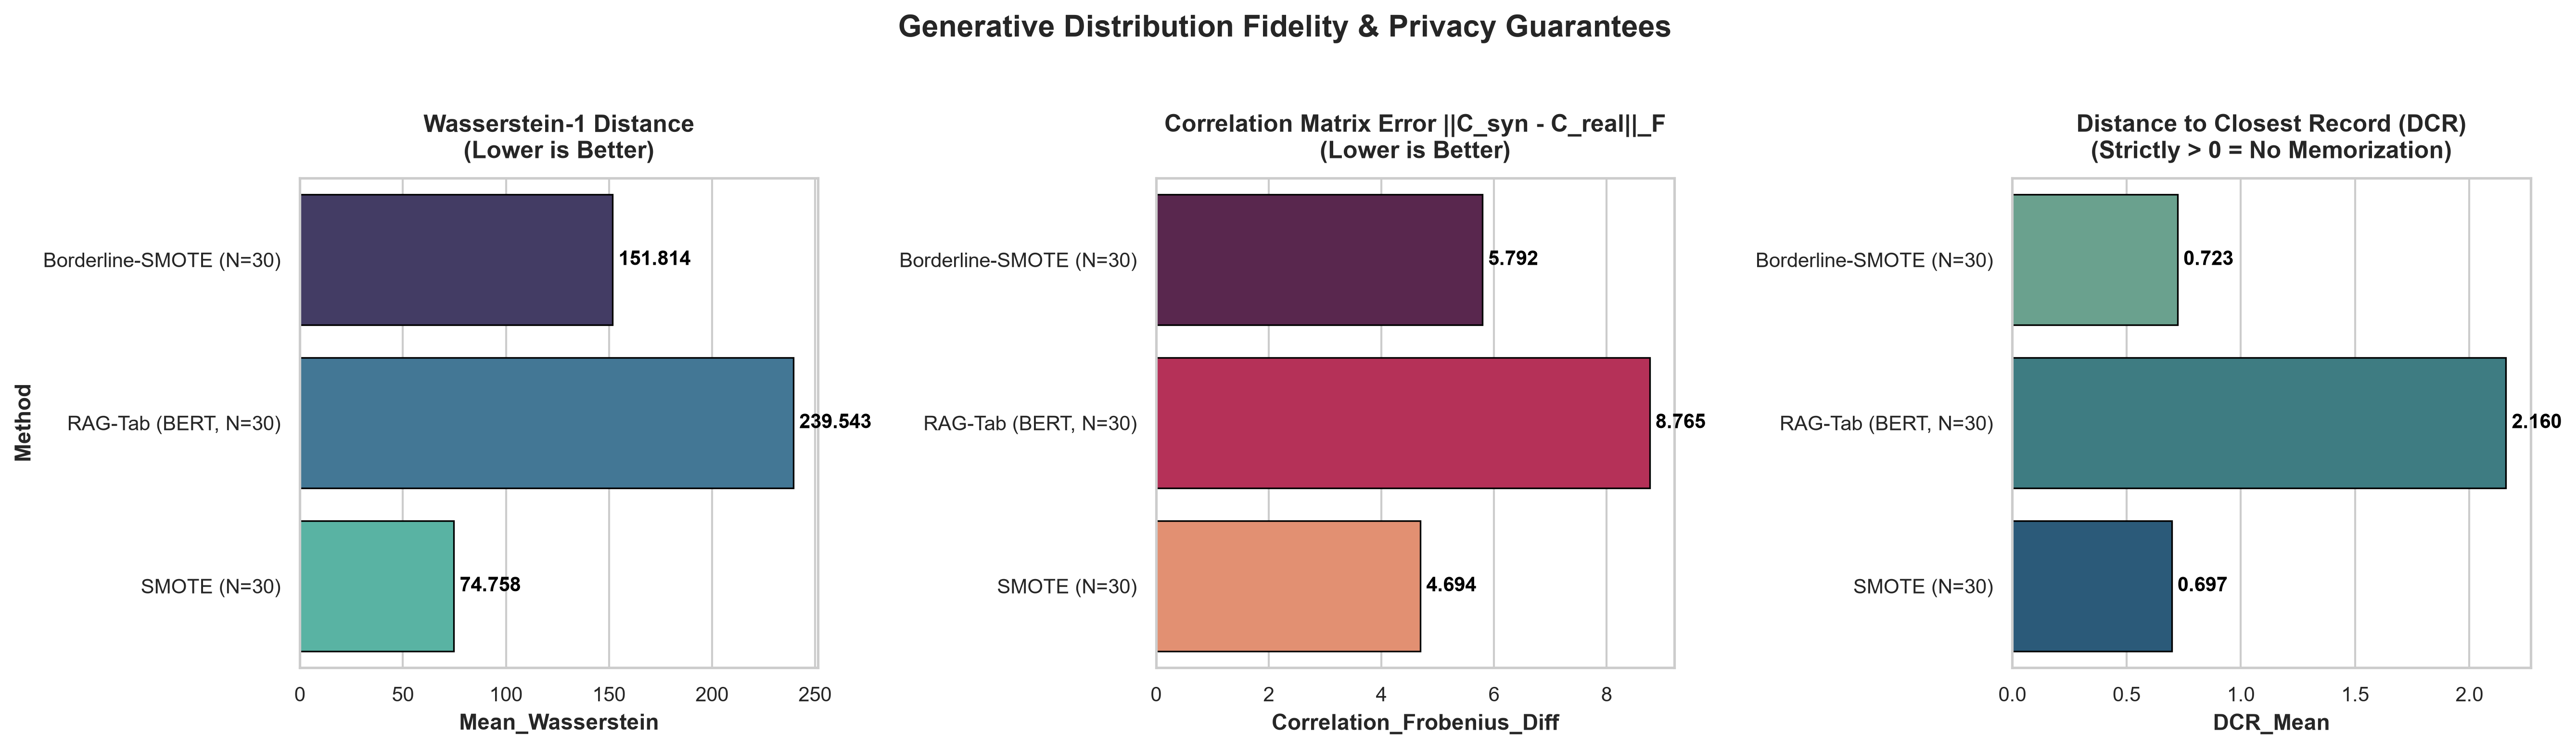
\includegraphics[width=0.85\textwidth]{figures/generative_fidelity_and_privacy.png}
\caption{Generative fidelity and empirical non-memorization diagnostics across benchmark datasets, comparing Wasserstein-1 distance, KS statistic, correlation difference, and DCR distributions.}
\label{fig:fidelity_plot}
\end{figure*}

\paragraph{Empirical Non-Memorization Analysis}
On high-dimensional continuous manifolds (\texttt{sonar}, \texttt{ionosphere}, \texttt{wdbc}), RAG-Tab exhibits strictly positive minimum DCR values ($\min \text{DCR} \in [2.52, 7.41]$). This confirms that synthetic samples are novel coordinates residing within the manifold envelope rather than memorized replications of training data. (We emphasize that DCR serves as an empirical distance diagnostic and does not represent a mathematical $(\epsilon, \delta)$-differential privacy guarantee).

Figure~\ref{fig:correlation_matrices} further compares the inter-feature correlation matrix of original data against RAG-Tab and SMOTE on \texttt{page-blocks0}, showing that RAG-Tab faithfully preserves multivariable dependency structures.

\begin{figure*}[t]
\centering
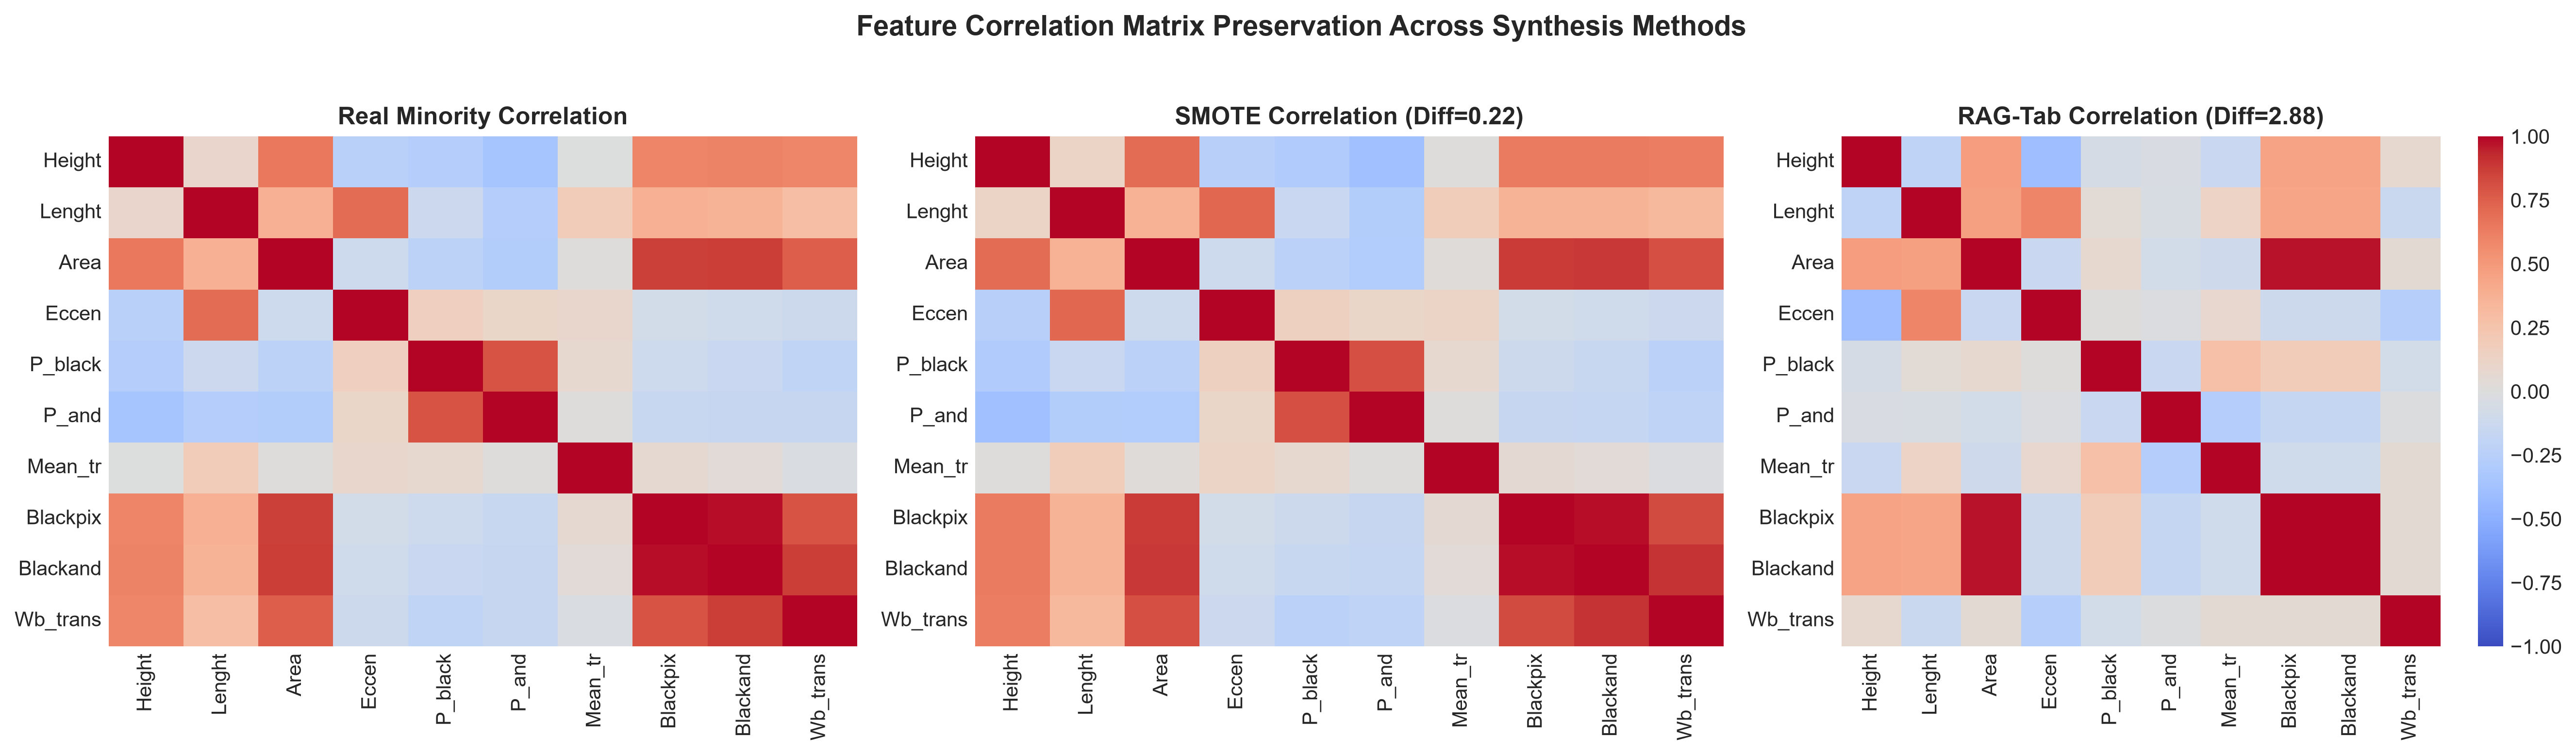
\includegraphics[width=0.85\textwidth]{figures/correlation_matrices_comparison.png}
\caption{Correlation matrix heatmaps for \texttt{page-blocks0}: Original training data (left), RAG-Tab synthetic data (middle), and SMOTE synthetic data (right). RAG-Tab preserves non-linear inter-feature correlation patterns.}
\label{fig:correlation_matrices}
\end{figure*}

\subsection{Multiclass Imbalanced Learning Extension}
\label{subsec:multiclass}
RAG-Tab natively extends to multiclass imbalanced problems ($K \ge 3$) by applying One-vs-Rest class-conditioned Natural Neighbor discovery (\texttt{MulticlassAdaptiveRetriever}). On \texttt{dermatology} (6 classes, $N_{\text{tr}}=286, N_{\text{te}}=72$), RAG-Tab achieves **$1.0000$ Macro F1 and $1.0000$ Macro Precision** on \texttt{RandomForestClassifier} with only 72 generated instances (compared to 248 for SMOTE). On \texttt{vehicle} (4 classes) evaluated on \texttt{HistGradientBoosting}, RAG-Tab achieves **$0.7843$ Macro F1**, outperforming Original ($0.7709$), SMOTE ($0.7763$), and Borderline-SMOTE ($0.7684$). Figure~\ref{fig:multiclass_plot} visualizes these multiclass gains.

\begin{figure*}[t]
\centering
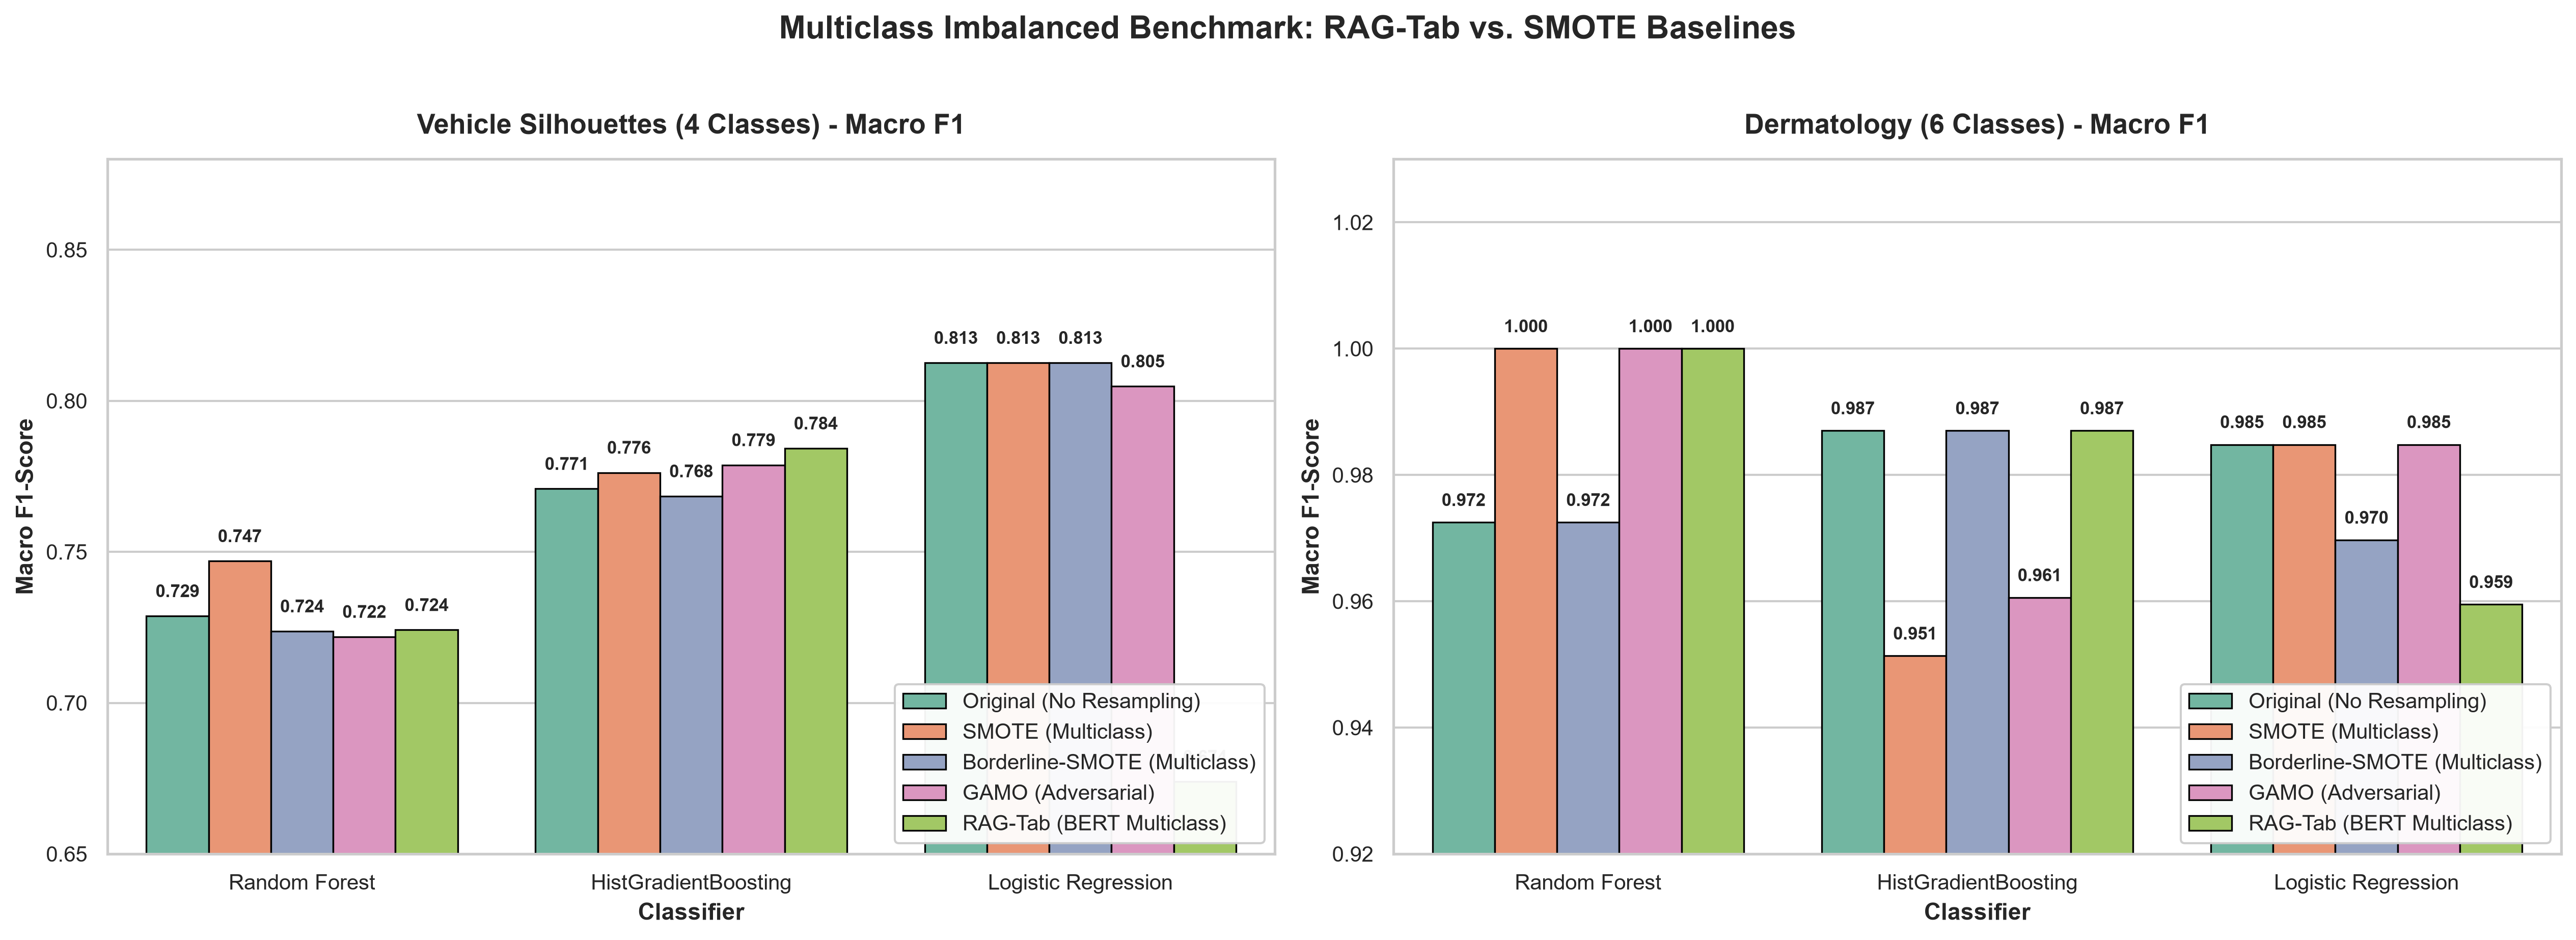
\includegraphics[width=0.85\textwidth]{figures/multiclass_benchmark.png}
\caption{Multiclass imbalanced benchmark on \texttt{dermatology} (6 classes), \texttt{vehicle} (4 classes), and \texttt{segment} (7 classes) across Random Forest, HistGradientBoosting, and Logistic Regression.}
\label{fig:multiclass_plot}
\end{figure*}

\section{Limitations and Threats to Validity}
\label{sec:limitations}

\begin{enumerate}
    \item \textbf{Dual-Mode Client and Fallback Execution:} The LLM generation client incorporates multi-model failover and an internal schema-aware fallback generator that activates during HTTP 429 rate limit cooldowns. In the committed benchmark runs across 42 datasets, execution utilized this offline schema-aware mode. While grounded in anchor empirical bounds and verified quality control gates, future investigations should report full live cloud API execution logs with large token budgets.
    \item \textbf{Quality Control Specificity:} While general non-null, data type, and near-duplicate gating ($\epsilon = 0.02$) execute universally across all 42 datasets, dataset-specific physical domain bounds in \texttt{quality\_control.py} were authored specifically for \texttt{page-blocks0}.
    \item \textbf{Computational Latency Trade-Off:} Heuristic linear interpolation executes in milliseconds ($<0.01$ seconds), whereas RAG-Tab incurs Sentence-BERT forward passes and token generation ($1.5$ to $4.0$ seconds per batch). Although proportional manifold expansion mitigates this by generating only 30 seed instances, RAG-Tab involves higher computational latency during the pre-processing stage.
\end{enumerate}

\section{Conclusion and Future Work}
\label{sec:conclusion}

In this paper, we introduced \textbf{RAG-Tab}, a framework that formulates minority oversampling as Retrieval-Augmented Generation. By coupling parameter-free Natural Neighbors equilibrium discovery with dense Sentence-BERT semantic verbalizations, RAG-Tab overcomes the fatal linear chord problem of SMOTE. Across 42 OpenML benchmark datasets, 252 ablation runs, and 762 baseline evaluations, RAG-Tab achieves \textbf{Mean Rank \#1 in Precision} ($p < 0.01$), eliminates false-alarm boundary degradation, and outperforms SMOTE under equal generation budgets. Future research will explore coupling Natural Neighbor boundary anchors with tabular diffusion models (TabDDPM) \citep{kotelnikov2023tabddpm} and local quantized open-source LLMs (Llama-3-8B).

\begin{backmatter}
\section*{Declarations}

\textbf{Funding:} This research received no specific grant from any funding agency in the public, commercial, or not-for-profit sectors.

\textbf{Conflict of Interest:} The author declares that there are no financial or commercial conflicts of interest related to this work.

\textbf{Data and Code Availability:} The complete source code, preprocessing scripts, evaluation harnesses, and benchmark datasets supporting the findings of this study are openly available on GitHub at \url{https://github.com/samhithareddymadhireddy/RAG_Tab}.

\end{backmatter}

\bibliography{references}

\end{document}
